
\documentclass[12pt,PhD,twoside,openright]{muthesis}

% Packages MU
\usepackage{verbatim}
\usepackage{graphicx}
\usepackage{url} % typeset URL's reasonably
\def\UrlBreaks{\do\/\do-}
\usepackage{listings}

\usepackage{pslatex} % Use Postscript fonts
\usepackage[toc]{}
% Uncomment this to use a glossary
% \usepackage[toc]{glossaries}
% \input{./glossary}
% \makeglossaries

%%%%%%%%%%%%%%%%%%%%%%
\usepackage{graphicx,latexsym}
\usepackage{amsmath}
\usepackage{amssymb,amsthm}
\usepackage{longtable,booktabs,setspace}
% \usepackage{chemarr} %% Useful for one reaction arrow, useless if you're not a chem major
% \usepackage[hyphens]{url}
% Added by CII
\usepackage[anythingbreaks]{}
\usepackage{hyperref}
\hypersetup{colorlinks = false}
\renewcommand{\UrlBreaks}{\do\/\do\a\do\b\do\c\do\d\do\e\do\f\do\g\do\h\do\i\do\j\do\k\do\l\do\m\do\n\do\o\do\p\do\q\do\r\do\s\do\t\do\u\do\v\do\w\do\x\do\y\do\z\do\A\do\B\do\C\do\D\do\E\do\F\do\G\do\H\do\I\do\J\do\K\do\L\do\M\do\N\do\O\do\P\do\Q\do\R\do\S\do\T\do\U\do\V\do\W\do\X\do\Y\do\Z\do\0\do\1\do\2\do\3\do\4\do\5\do\6\do\7\do\8\do\9\do\%\do\.\do\-}

\renewcommand{\chapterautorefname}{Chapter}

\usepackage{lmodern}
\usepackage{float}
\floatplacement{figure}{H}
% End of CII addition
\usepackage{rotating}


\usepackage{natbib}
%%% --- The following two lines are what needs to be added --- %%%
%\setcounter{biburllcpenalty}{7000}
%\setcounter{biburlucpenalty}{8000}
% Comment out the natbib line above and uncomment the following two lines to use the new
% biblatex-chicago style, for Chicago A. Also make some changes at the end where the
% bibliography is included.
%\usepackage{biblatex-chicago}
%\bibliography{thesis}


% Added by CII (Thanks, Hadley!)
% Use ref for internal links
% \renewcommand{\hyperref}[2][???]{\autoref{#1}}
% \def\chapterautorefname{Chapter}
% \def\sectionautorefname{Section}
% \def\subsectionautorefname{Subsection}
% End of CII addition

% Added by CII
\usepackage{caption}
% \captionsetup{width=5in}
% End of CII addition

% \usepackage{times} % other fonts are available like times, bookman, charter, palatino

% Syntax highlighting #22
  \usepackage{color}
  \usepackage{fancyvrb}
  \newcommand{\VerbBar}{|}
  \newcommand{\VERB}{\Verb[commandchars=\\\{\}]}
  \DefineVerbatimEnvironment{Highlighting}{Verbatim}{commandchars=\\\{\}}
  % Add ',fontsize=\small' for more characters per line
  \usepackage{framed}
  \definecolor{shadecolor}{RGB}{248,248,248}
  \newenvironment{Shaded}{\begin{snugshade}}{\end{snugshade}}
  \newcommand{\AlertTok}[1]{\textcolor[rgb]{0.94,0.16,0.16}{#1}}
  \newcommand{\AnnotationTok}[1]{\textcolor[rgb]{0.56,0.35,0.01}{\textbf{\textit{#1}}}}
  \newcommand{\AttributeTok}[1]{\textcolor[rgb]{0.77,0.63,0.00}{#1}}
  \newcommand{\BaseNTok}[1]{\textcolor[rgb]{0.00,0.00,0.81}{#1}}
  \newcommand{\BuiltInTok}[1]{#1}
  \newcommand{\CharTok}[1]{\textcolor[rgb]{0.31,0.60,0.02}{#1}}
  \newcommand{\CommentTok}[1]{\textcolor[rgb]{0.56,0.35,0.01}{\textit{#1}}}
  \newcommand{\CommentVarTok}[1]{\textcolor[rgb]{0.56,0.35,0.01}{\textbf{\textit{#1}}}}
  \newcommand{\ConstantTok}[1]{\textcolor[rgb]{0.00,0.00,0.00}{#1}}
  \newcommand{\ControlFlowTok}[1]{\textcolor[rgb]{0.13,0.29,0.53}{\textbf{#1}}}
  \newcommand{\DataTypeTok}[1]{\textcolor[rgb]{0.13,0.29,0.53}{#1}}
  \newcommand{\DecValTok}[1]{\textcolor[rgb]{0.00,0.00,0.81}{#1}}
  \newcommand{\DocumentationTok}[1]{\textcolor[rgb]{0.56,0.35,0.01}{\textbf{\textit{#1}}}}
  \newcommand{\ErrorTok}[1]{\textcolor[rgb]{0.64,0.00,0.00}{\textbf{#1}}}
  \newcommand{\ExtensionTok}[1]{#1}
  \newcommand{\FloatTok}[1]{\textcolor[rgb]{0.00,0.00,0.81}{#1}}
  \newcommand{\FunctionTok}[1]{\textcolor[rgb]{0.00,0.00,0.00}{#1}}
  \newcommand{\ImportTok}[1]{#1}
  \newcommand{\InformationTok}[1]{\textcolor[rgb]{0.56,0.35,0.01}{\textbf{\textit{#1}}}}
  \newcommand{\KeywordTok}[1]{\textcolor[rgb]{0.13,0.29,0.53}{\textbf{#1}}}
  \newcommand{\NormalTok}[1]{#1}
  \newcommand{\OperatorTok}[1]{\textcolor[rgb]{0.81,0.36,0.00}{\textbf{#1}}}
  \newcommand{\OtherTok}[1]{\textcolor[rgb]{0.56,0.35,0.01}{#1}}
  \newcommand{\PreprocessorTok}[1]{\textcolor[rgb]{0.56,0.35,0.01}{\textit{#1}}}
  \newcommand{\RegionMarkerTok}[1]{#1}
  \newcommand{\SpecialCharTok}[1]{\textcolor[rgb]{0.00,0.00,0.00}{#1}}
  \newcommand{\SpecialStringTok}[1]{\textcolor[rgb]{0.31,0.60,0.02}{#1}}
  \newcommand{\StringTok}[1]{\textcolor[rgb]{0.31,0.60,0.02}{#1}}
  \newcommand{\VariableTok}[1]{\textcolor[rgb]{0.00,0.00,0.00}{#1}}
  \newcommand{\VerbatimStringTok}[1]{\textcolor[rgb]{0.31,0.60,0.02}{#1}}
  \newcommand{\WarningTok}[1]{\textcolor[rgb]{0.56,0.35,0.01}{\textbf{\textit{#1}}}}




% if you're writing a thesis in an interdisciplinary major,
% uncomment the line below and change the text as appropriate.
% check the Senior Handbook if unsure.
%\thedivisionof{The Established Interdisciplinary Committee for}
% if you want the approval page to say "Approved for the Committee",
% uncomment the next line
%\approvedforthe{Committee}

% Added by CII
%%% Copied from knitr
%% maxwidth is the original width if it's less than linewidth
%% otherwise use linewidth (to make sure the graphics do not exceed the margin)
% \makeatletter
% \def\maxwidth{ %
%   \ifdim\Gin@nat@width>\linewidth
%     \linewidth
%   \else
%     \Gin@nat@width
%   \fi
% }
% \makeatother

% \renewcommand{\contentsname}{Table of Contents}
% End of CII addition

% \setlength{\parskip}{0pt}

% Added by CII
% 
\providecommand{\tightlist}{%
  \setlength{\itemsep}{0pt}\setlength{\parskip}{0pt}}

	\usepackage{amsmath}
 \usepackage{ulem}

\newlength{\cslhangindent}
\setlength{\cslhangindent}{1.5em}
\newenvironment{cslreferences}%
  {}%
  {\par}
  

\begin{document}

\title{Multi-State Clinical Prediction Models in Renal Replacement Therapy}
\author{Michael Andrew Barrowman}
\principaladviser{}
\faculty{}
\school{}
\beforeabstract

\prefacesection{Abstract}
The preface pretty much says it all.

\par

Second paragraph of abstract starts here.

\afterabstract

\prefacesection{Acknowledgements}

\begingroup

\setlength{\parskip}{15pt}
\setlength{\parindent}{0pt}

\endgroup
\afterpreface

\newcommand{\txt}[1]{\textrm{#1}}

\def\logit{\textrm{logit}}

\newcommand{\sfrac}[2]{\;^{#1}/_{#2}}

\hypertarget{page-one}{%
\chapter{Page One}\label{page-one}}

HTML Output is FALSE and LaTeX output is incorrectly FALSE

Testing new line

\hypertarget{chap-lit-report}{%
\chapter{Literature Report}\label{chap-lit-report}}

\hypertarget{introduction}{%
\section{Introduction}\label{introduction}}

lorem ipsum blah blah blah

\hypertarget{clinical-prediction-models}{%
\section{Clinical Prediction Models}\label{clinical-prediction-models}}

The idea of prognosis dates back to ancient Greece with the work of Hippocrates {[}1{]} and is derived from the Greek for ``know before'' meaning to forecast the future. Within the sphere of healthcare, it is definde as the risk of future health outcomes in patients, particularly patients with a certain disease or health condition. Prognosis allows clinicians to provide patients with a prediction of how their disease will progress and is uaully given as a probability of having an event in a prespecified number of years. For example, QRISK3 {[}2{]} provides a probability that a patient will have a heart attack or stroke in the next 10 years. Prognostic research encompasses any work which enhances the field of prognosis, whether through methodological advancements, field-specific prognostic modelling or educational material designed to improve general knowledge of prognosis. Prognostic models come under the wider umbrella of predictive models which also includes diagnostic models; because of this most of the keys points in the field or prognostic modeling can be applied to diagnostic models with little to no change.

Prognosis allows clinicians to evaluate the natural history of a patient (i.e.~the course of a patient's future without any intervention) in order to establish the ffect of screening for asymptomatic diseases (such as with mammograms{[}3{]}). Prognosis research can be used to develop new definitions of diseases, whether a redefinition of an existing disease (such as the extension to th definition of myocardial infarction to include non-fatal events {[}4{]}) or a previously unknown subtype of a disease (such as Brugada syndrome as a type of cardiovascular disease{[}5{]})

In general, prognosis research can be broken down into four main categories, with three subcategories {[}6{]}:
\begin{itemize}
\tightlist
\item
  Type I: Fundamental prognosis research {[}3{]}
\item
  Type II: Prognostic factor research {[}7{]}
\item
  Type III: Prognostic model research {[}8{]}
  \begin{itemize}
  \tightlist
  \item
    Model development {[}9{]}
  \item
    Model validation {[}10{]}
  \item
    Model impact evaluation {[}11{]}
  \end{itemize}
\item
  Type IV: Stratified Medicine {[}12{]}
\end{itemize}
For a particular outcome, prognostic research will usually progress through these types, beginning with papers designed to evaluate overall prognosis within a whole population and then focusing in on more specificity and granularity towards individualised, causal predictions.

The model development and validation will usually occur in the same paper {[}13{]}, {[}14{]}. studies into all three of the subcategories of prognostic model research \emph{should} be completed before a model is used in clinical practice {\textbf{???}}, although this does not always occur {[}8{]}. External validation is considered by some to be more important than the actual deviation of the model as it demonstrates generalisability of the model {\textbf{???}}, whereas a model on it's own may be highly susceptible to overfitting {[}\textbf{Cite: Something}{]}.

\hypertarget{fundamental-prognosis-research}{%
\subsection{Fundamental Prognosis Research}\label{fundamental-prognosis-research}}

{[}\textbf{What is it? Old definition is incorrect, so will need to write this fresh}{]}

\hypertarget{prognostic-factor-research}{%
\subsection{Prognostic Factor Research}\label{prognostic-factor-research}}

The aim of prognostic factor research (Type II) is to discover which factors are associated with disease progression. This allows for the general attribution of relationships between predictors and clinical outcomes.

Predictive factor research can give researchers and clinicians an idea of which patient factors are important when assessing a disease. It is vital to the development of clinical predictive models as without an idea of what covariates \emph{can} affect an outcome, we cannot figure out which variables \emph{will} affect the outcome. For example, {[}\textbf{xxxx}{]} demonstrated that {[}\textbf{xxxx}{]} is correlated with {[}\textbf{xxxx}{]}, which subsequently used as a covariate in the development of the {[}\textbf{xxxx}{]} model. Note the use of the word correlate here as prognostic relationships do not have to be causal ones {[}\textbf{Cite: Something}{]}. These factors may indeed represent an underlying causal pathway, but this is not a requirement and it would require aetiological methods to discern whether it were causal or not. For example, when predicting {[}\textbf{xxxx}{]}, we can demonstrate that {[}\textbf{xxxx}{]} is a prognostic factor, {[}however since the arrow of causation is {[}\textbf{xxxx}{]}{]} {[}\textbf{OR}{]} {[}however since {[}\textbf{xxxx}{]} causes both {[}\textbf{xxxx}{]} and {[}\textbf{xxxx}{]}{]}, the relationship is prognostic, but not causal. {[}\textbf{Previously used Apgar score here, reference 40}{]}

Counter to the idea that prognostic factors aren't always causal, they are \emph{always} confounding factors for the event they predict. Thue prognostic factors should be taken into account when planning clinical trials as if they are wildly misbalanced across the arms (or not accounted for in some other manner), they can cause biases in the results {[}7{]}. Sometimes these factors are so strong that adjusting the results of a clinical trial by the factor can affect, or even reverse the interpretation of the results {\textbf{???}}. If a prognostic factor is causal, then by directly affecting the factor, it can causally affect the outcome. By discovering new prognostic factors, and investigating their causality, we can potentially open the door to new directions of attack for treatments.

It is unfortunate, however, that Riley at al {\textbf{???}} found that only 35.5\% of prognostic factor studies in paediatric oncology actually reported the size of the effect of the prognostic factor they reported on. This means that very little information can be drawn from these studies. It is also important that prognostic factor research papers consider and report on the implications of the factor they assess such as healthcare costs. These kinds of implications are rarely assessed, especially when compared to drugs or interventions {[}7{]}.

\hypertarget{prognostic-model-research}{%
\subsection{Prognostic Model Research}\label{prognostic-model-research}}

Predictive factors can be combined into a predictive model, which is a much more specific measurement of the effect of a factor on an outcome {[}8{]} and they are deigned to augment the job of a clinician; and not to completely replace them {[}11{]}. Diagnostic prediction model can be used to indicate whether a patient is likely to need further testing to establish the presence of a disease {[}13;\textasciitilde moons\_transparent\_2015{]}. Prognostic prediction models can be used to decide on further treatment for that patient, whether as a member of a certain risk group, or under a stratied medicine approach {[}13{]}, {[}14{]}. Outcomes being assessed in a prediction model should be directly relevant to the patient (such as mortality) or have a direct causal relationship with something that is {[}11{]}. There is a trend of researchers focusing on areas of improvement that are of less significance to the patient than it is to a physician {[}\textbf{Cite: LR - 18}{]}. For example, older patient's might prefer to have an improved quality of life than an increase in life expectancy, and thus models should be developed to account for this.

Creating a clinicaly useful model is not as simple as just using some availble data to develop a model, despite what a lot of researchers seem to believe {[}\textbf{Cite: Something}{]}. To quote Steyerberg et al {[}8{]}. " To be useful for clinicia,s a prognostic model needs to provide validated and accurate predictions and to improve patient outcomes and cost-effectiveness of care". This means that, although a mdel might appear to be useful, its effectiveness is only relevant to the population it was developed in. If your population is different, then the model will behave differently. Bleeker {\textbf{???}} developed a model to predict bacterial infections in febrile children with an unknown source. The model scored well when assessed for the predictive value in the development dataset, however it scored much worse in an external dataset implying that, though it worked well in the development population, it would be unwise to apply it to a new population.

\hypertarget{model-development}{%
\subsubsection{Model Development}\label{model-development}}

The first stage of having a useful model is to develop one. Clinical predictive models can take a variety of forms, such as logistic regression, cox models or some kind of machine learning. Regardless of the specific model type being used, there are certain universal truths than should be held up during model development which will be discussed here. The size of the dataset being used is of vital importance as it can combat overfitting of the data, but so is choosing which prognostic factors to be included in the final model. This section will discuss various ideas that researchers need to account for when developing a model from any source and can be applied to any model type.

By considering a multivariable approach to prediction models (as opposed to a univariable one), researchers can consider different combinations of predictive factors, usually refered to as potential predictors {[}\textbf{Cite: LR - 2}{]}. These can include factors where a direct relationship with the disease can be clearly seen, such as tumour size in the prediction of cancer mortality {[}\textbf{Cite: LR - 5}{]}, or ones which could have a more general effect on overall health, such as socioeconomic and ethnicity variables {[}\textbf{Cite: LR - 55}{]}. By ignoring any previous assumptions about a correlation between these potential predictors and the outcome of interest, we can cast a wider net in our analysis allowing us to catch relationships that might have otherwise been lost {[}\textbf{Cite: LR - 56}{]}. Prediction models should take into account as many predictive factors as possible. Demographic data should also be included as these are often found to be confounding factors, variables such as ethnicity and social deprivation risk exacerbating the existing inequality between groups r LR(7)`.

When developing a predictive model, the size of the dataset being used in an important consideration. A typical ``rule of thumb'' is to have at least 10 events for every potential predictor {[}\textbf{Cite: LR - 57, 58}{]}, know as the Events-per-Variable (EPV). Recently, this number has been superseded by a methods to evaluate a specific required sample size {[}\textbf{Cite: Riley, EPV work}{]}. If there aren't enough events to satisfy this criteria, then some potential predictors should be eliminated before any formal analysis takes place (for example using clinical knowledge) {[}\textbf{Cite: LR - 59}{]}. In general, it is also recommended that this development dataset contain at least 100 events (regardless of number of potential predictors) {[}\textbf{Cite: LR - 39, 60, 61}{]}. A systematic review by Counsell et al {[}\textbf{Cite: LR - 62}{]} found that out of eighty-three prognostic models for acute stroke, less than 50\% of them had more than 10 EPV, and the work by Riley et al {[}\textbf{Cite: riley EPV Work}{]} showed that less that {[}\textbf{Pull example from Riley EPV}{]}. Having a low EPV can lead to overfitting of the model which is a concern associated with having a small data set. Overfitting leads to a worse prediction when the model is used on a new population which essentially makes the model useless{[}\textbf{Cite: LR - 34}{]}. However, just because a dataset is large does not imply that it will be a \emph{good} dataset if the quality of the data is lacking {[}\textbf{Cite: LR - 39}{]}. Having a large amount of data can lead to predictors being considered statistically significant when in reality they only add a small amount of information to the model {[}\textbf{Cite: LR - 39}{]}. The size of the effect of a predictor should therefore be taken into account in the final model and, if beneficial, some predictors can be dropped at the final stage.

Large datasets can be used for both development and validation if an effective subset is chosen. This subset should not be random or data driven and should be decided before data analysis is begun {[}\textbf{Cite: LR - 39}{]}. Randomly splitting a dataset set into a training set (for development) and a testing set (for internal validation) can result in optimistic results in the validation process in the testing set. This is due to the random nature of the splitting causing the two populations to be too exchangeable, which is similar to the logic behind the splitting of patients in a Randomised Control Trial (RCT). Splitting the population by a specific characteristic (such as geographic location or time period) can result in a better internal validation {[}\textbf{Cite: LR - 35, 63}{]}. Derivation of the QRISK2 Score {[}\textbf{Cite: LR - 7}{]} (known later as QRISK2-2008) randomly assigned two thirds of practices to the derivation dataset and the remainder to the validation dataset {[}\textbf{Check how QRISK3 Does this}{]}. The NPI model {[}\textbf{Has this been mentioned?}{]} was trained on the first 500 patients admitted to Nottingham City Hospital after the study began {[}\textbf{Cite: LR - 5}{]} and later validated on the next 320 patients to be admitted {[}\textbf{Cite: LR - 64}{]}, this validation was not performed at the same time as the initial development and is thus an external validation.

If a sufficient amount of data is available and it has been taken from multiple sources (practices, clinics or studies), then it should be clustered to account for heterogeneity across sources {[}\textbf{Cite: LR - 65}{]}. It is important that any sources of potential variability are identified (such as heterogeneity between centres) as this can have an impact on the results of any analysis {[}\textbf{Cite: LR - 1, 39}{]}. Heterogeneity is particularly high when using multiple countries as a source of data {[}\textbf{Cite: LR - 66}{]} or if a potential predictor is of a subjective nature, which leads to discrepancies between assessors {[}\textbf{Cite: LR - 67}{]}. Overlooking of this clustering can lead to incorrect inferences {[}\textbf{Cite: LR - 65}{]}. The generalisability of the sources of data should also be considered in the development of a model. For example, the inclusion and exclusion criteria of an RCT can greatly reduce generalisability if used as a data source {[}11{]}.

A prediction model researcher needs to select clinically relevant potential predictors for use in the development of the model {[}\textbf{Cite: LR - 34}{]}. Once chosen, researchers need to be very specific about how these variables are treated. Any adjustments from the raw data should be reported in detail

\hypertarget{model-validation}{%
\subsubsection{Model Validation}\label{model-validation}}

\hypertarget{impact-evaluation}{%
\subsubsection{Impact Evaluation}\label{impact-evaluation}}

\hypertarget{stratified-medicine}{%
\subsection{Stratified Medicine}\label{stratified-medicine}}

\hypertarget{examples}{%
\subsection{Examples}\label{examples}}

\hypertarget{competing-risks-multi-state-models}{%
\section{Competing Risks \& Multi-State Models}\label{competing-risks-multi-state-models}}

\hypertarget{chap-scoping-review}{%
\chapter{The Application of Multi-State Methods to Develop Clinical Prediction Models Designed for Clinical Use - A Scoping Review}\label{chap-scoping-review}}

\hypertarget{introduction-1}{%
\section{Introduction}\label{introduction-1}}

eHealthcare is moving towards a more data-driven approach to decision making, exploiting the variety of data sources collected as part of routine care {[}1{]}. This increases efficiency, which is becoming increasingly vital as patients are living longer and requiring more care, while budgets are being reduced {[}2{]}, {[}3{]}. Correspondingly, there has been a shift towards primary prevention, rather than purely treating disease as it arises {[}4{]} therefore clinical prediction models (CPMs) are more relevant than ever before {[}5{]}.

Prognostic CPMs (those that predict the future) allow end-users to estimate an individual's probability/risk of experiencing an outcome of interest within a certain timeframe. CPMs are algorithms that relate a set of prognostic factors to the risk of a chosen outcome {[}6{]}, often using multivariable regression. They can provide predictions of the future course of an illness and provide evidence for the commencement of medical interventions {[}7{]}.

Along with this overall increase in importance, different methods of producing CPMs are also being used, and each makes different assumptions, and models at different levels of granularity. One of these methods is the Multi-State Model (MSM), an extension to traditional survival analysis wherein patients exist in one of many distinct states at any given time and can transition between them (these individual transitions are akin to that of traditional survival analysis) {[}8{]}. A subset of MSMs is that of a Competing Risks model, where patients can only move from a single initial state to many absorbing states without any intermediate or transient states. A huge advantage of Multi-State CPMs, and indeed, Competing Risks CPMs, is that they can provide predictions for multiple outcomes with MSMs going further by allowing the prediction of multiple pathways to that outcome, whereas traditionally developed models only provide predictions for a single end-point.

However, little is known about how widely these types of models are implemented in clinically relevant prognostic research. Therefore, we here aim to document a scoping review protocol that will intend to uncover any prediction models using MSMs that have been developed for clinical use. As part of the process of this investigation, we will also document how many CPMs account for Competing Risks alone. We define a scoping review as described by Arksey and O'Malley {[}9{]} , which is similar to a systematic review, but with less formal outline for the analysis and synthesis of literature {[}10{]}. By assessing how MSMs have currently been applied in this field, we aim to describe the landscape of their current use, the context in which they are being used and discuss ways in which their use, application and uptake can be improved. To the best of our knowledge, a review such as this for Multi-State Models has never been performed.

\hypertarget{methods}{%
\section{Methods}\label{methods}}

\[ 
A= \pi r^2
\]

\hypertarget{scope-of-review}{%
\subsection{Scope of Review}\label{scope-of-review}}

This review will cover articles related to the development of Multi-State Clinical Prediction models designed for clinical use. It will not include models that were developed solely for demonstrations of novel methodological improvements in the field of clinical prediction modelling and/or multi-state modelling. Article inclusion will be based on the screening of the article text and interpretation of its aims, primary distinction will be made on whether an existing dataset is used as a core part of the article or as a subsidiary example. It will include articles that validate previously developed models and those that review existing models, only so far as to use them to find the original development article (a method known as Snowballing).

As this analysis will follow the style of a scoping review; the final paper will adhere to the PRISMA-ScR guidelines {[}11{]}, which were set out to extend the traditional PRISMA guidelines to a Scoping Review setting.

Models which focus only on a competing risks scenario (whether directly or simply adjusting for competing risks) will not be analysed in detail, however to avoid missing possible Multi-State Models, we will only omit these at the final stage of screening (See below). This will also allow for a brief description of how many CR models exist compared to the MSM models to be analysed in detail in this review.

As per the definitions set out by the PROGRESS research group, prognostic research is split into four overarching themes/types:
\begin{itemize}
\tightlist
\item
  Type I - Fundamental Prognosis Research {[}12{]}
\item
  Type II - Prognostic Factor Research {[}13{]}
\item
  Type III - Prognostic Model Research {[}14{]}
\item
  Type IV - Stratified Medicine Research {[}15{]}
\end{itemize}
As such, we will be focusing on papers of Type III {[}14{]}. Articles related to the other types of prognostic research often develop a model within their work, but since the intent of these papers is to investigate overall outcomes, effects of an individual factor or interactive effects of treatments in individuals, they are considered disjoint from CPM development and so they will not be included in our analysis.

\hypertarget{initial-search-strategy}{%
\subsection{Initial Search Strategy}\label{initial-search-strategy}}

\hypertarget{search-terms}{%
\subsubsection{Search Terms}\label{search-terms}}

To ensure we cover as much of the medical literature as possible, we will use the Ovid search engine to search two databases:
\begin{itemize}
\tightlist
\item
  EMBASE (1974 to 2018 December 31)
\item
  Ovid MEDLINE and Epub Ahead of Print, In-Process \& Other Non-Indexed Citations, Daily and Versions 1946 to December 31, 2018
\end{itemize}
We will use a standard set of terms designed by Ingui \& Rogers {[}16{]} and added to by Geersing et al {[}17{]} used for searching for clinical prediction related literature. We will also extend this by including search terms relating to time-to-event outcomes and/or survival analysis that were defined by the authors, and which aim to broaden our search (see table 1). This will be combined by a set of search terms designed to filter for MSMs and/or CRs.

These novel MSM/CR terms include ``fine adj2 gray'' to include papers which use the Fine \& Gray subdistribution proportional hazard method {[}18{]}. It will also include``semimarkov or semi markov'' to include articles which specify that the model adopts a semi-Markov perspective, which is common amongst MSMs {[}8{]}. However, we chose not to include the term ``markov'' alone as it is considered to be too unspecific to be of use (a la search for ``model'' alone when finding clinical prediction models). The full search details can be found in table 2.

We believe that the broadness of our search terms allows for high sensitivity in our results and will therefore provide a larger and more comprehensive pool of papers than using a more specific set of search terms.

{[}\textbf{Insert Table from paper}{]}

\hypertarget{validation-set-of-articles}{%
\subsubsection{Validation set of articles}\label{validation-set-of-articles}}

To ensure that our search strategy is satisfactory, we will compare our results to a set of Validation papers. These are papers that we are already aware of that satisfy our inclusion/exclusion criteria and which therefore should be included in our analysis. We will compare the results of our initial search with this set of papers to ensure that all of the Validation set appear in our results. If they do not, then we will adjust our search strategy iteratively increasing sensitivity and improving the reach of our search until all Validation papers are included. The set of Validation papers is as follows:
\begin{itemize}
\tightlist
\item
  \emph{Estimation and Prediction in a Multi-State Model for Breast Cancer}, Putter et al, 2006 {[}20{]}
\item
  \emph{A Multi-State Model to Predict Heart Failure Hospitalizations and All-Cause Mortality in Outpatients With Heart Failure With Reduced Ejection Fraction: Model Derivation and External Validation}, Upshaw et al, 2016 {[}21{]}
\item
  \emph{Predicting timing of clinical outcomes in patients with chronic kidney disease and severely decreased glomerular filtration rate}, Grams et al, 2018 {[}22{]}
\item
  \emph{Estimating transition probability of different states of type 2 diabetes and its associated factors using Markov model}, Nazari et al, 2018 {[}23{]}
\item
  \emph{Advantages of a multi-state approach in surgical research: how intermediate events and risk factor profile affect the prognosis of a patient with locally advanced rectal cancer}, Manzini et al, 2018 {[}24{]}
\end{itemize}
\hypertarget{filtering}{%
\subsection{Filtering}\label{filtering}}

Once the initial set of articles has been found, these will be filtered at various degrees of granularity to focus on papers which are included in the scope of our review as per our inclusion/exclusion criteria. We will also define which papers will be used only for the snowballing process, but will not be used as part of our analysis.

\hypertarget{inclusionexclusion-criteria}{%
\subsubsection{Inclusion/Exclusion Criteria}\label{inclusionexclusion-criteria}}

Inclusion
\begin{itemize}
\tightlist
\item
  Type III Prognostic Study Papers (i.e.~those developing a clinical prediction model) {[}14{]}
\item
  Papers which use a Multi-State Model framework to provide individual level patient predictions
\end{itemize}
Exclusion
\begin{itemize}
\tightlist
\item
  Papers that develop overall population level predictions (Type I)
\item
  Papers focused on identification of prognostic factors (Type II)
\item
  Papers that investigate stratified medicine (Type IV)
\item
  Papers that only develop Competing Risks models
\item
  Papers designed to describe methodological models with or without clinical application used only for an example
\end{itemize}
\hypertarget{stages}{%
\subsubsection{Stages}\label{stages}}

The filtering of the results will be performed in three stages:
1. Title (MB)
2. Abstract (MB with 20\% replication by DJ)
3. Full Paper (MB with 20\% replication by DJ)

Filtering will begin with an initial check through all titles to assess whether it is believed that the paper may be relevant to the review. This will help to omit a large amount of papers that were incorrectly returned by the broad search strategy. To ensure the review remains as sensitive as possible, only papers where it is abundantly clear that they violate an inclusion/exclusion criteria will be removed at this stage.

A second filter will be performed on the abstracts of the remaining articles and removed papers will be classified by the reason for their omission. To allow for faster data extraction, a final glancing filter will also be performed over the full papers to again reduce the numbers of collated papers in the final review and reduce the likelihood of removing papers at the analysis stage. To ensure robustness of this filtering, both of these stages will be replicated by a second reviewer (DJ) in a randomly selected 20\% of the abstracts and papers and differences will be discussed internally. At this point, models focusing solely on competing risks (i.e.~those without a transient state) will be filtered out.

\hypertarget{data-extraction}{%
\subsection{Data Extraction}\label{data-extraction}}

To study the use of Multi-State Clinical Prediction Models from a quantitative perspective, certain vital data points will be extracted from the extant models. These measurements can be grouped as to what element of the prediction model they are evaluating:
* Clinically Relevant points
* Number of patients
* Clinical setting (i.e.~primary vs secondary care, geographic setting)
* Field of study (e.g.~cardiovascular, renal, etc.)
* Summary of patient demographics (i.e.~inclusion/exclusion criteria)
* Outcomes being predicted
* Multi-State Model details
* Number of States and what they are
* Shape/Structure of the model (i.e.~how patients can transition between states)
* How were relevant variables chosen?
* Transition assumptions (e.g.~parametric vs non-parametric, PH assumption, etc\ldots)
* Stated justification for, and reported benefits of an MSM versus traditional methods.
* Predictive Ability
* Timeframe (e.g.~single time point(s), continuous time prediction, dynamic prediction, etc\ldots)
* What validation was performed (None vs.~Internal (bootstrap, CV, etc.) vs.~External)
* Comparisons to current guidelines
* Assessment of Bias of their model (using PROBAST)
* Utilisation of the TRIPOD Guidelines (e.g.~Was it referenced? Was it adhered to?)
* Prominence information
* Number of citations (although not clinically relevant, it is relevant to understanding the model's utilisation)
* Year of publication (again, not clinically relevant, but useful to spot any time trends in prominence and/or quality)
The data extracted at this stage will be checked by DJ in 20\% of the papers to confirm results for the analysis

\hypertarget{reporting}{%
\subsection{Reporting}\label{reporting}}

The search and filtering strategy will be depicted with a modified PRISMA flow diagram {[}30{]}, which includes papers found by Snowballing and how they are included in the filtration process, see figure 1.

{[}\textbf{Add in PRISMA}{]}

A table of the extracted information will be included with the paper, depending on the number of results, this may be supplementary material. This information will also be summarised and analysed both quantitatively and qualitatively. For example, as the Illness-Death model {[}8{]} is simple and common amongst multi-state models, we will count how many of the MSCPMs use this structure as well as the other most common structures used. Any direct comparisons that can be made between predictions of this type (i.e.~from the same field with the same outcomes) will be described.

\hypertarget{chap-Conf-CR}{%
\chapter{How unmeasured confounding in a competing risks setting can affect treatment effect estimates in observational studies}\label{chap-Conf-CR}}

\hypertarget{background}{%
\section{Background}\label{background}}

Well-designed observation studies permit researchers to assess treatment effects when randomisation is not feasible. This may be due to cost, suspected non-equipoise treatments or any number of other reasons {[}1{]}. While observational studies minimise these issues by being cheaper to run and avoiding randomisation (which, although unknown at the time, may prescribe patients to worse treatments), they are potentially subject to issues such as unmeasured confounding and increased possibility of competing risks (where multiple clinically relevant events occur). Although these issues can arise in any study, Randomised Controlled Trials (RCTs) attempt to mitigate these effects by using randomisation of treatment and strict inclusion/exclusion criteria. However, the estimated treatment effects from RCTs are of potentially limited generalisability, accessibility and implementability {[}2{]}.

A confounder is a variable that is a common cause of both treatment and outcome. For example, a patient with a high Body Mass Index (BMI) is more likely to be prescribed statins {[}3{]}, but are also more likely to suffer a cardiovascular event. These treatment decisions can be affected by variables that are not routinely collected (such as childhood socio-economic status or the severity of a comorbidity {[}4{]}. Therefore, if these variables are omitted form (or unavailable for) the analysis of treatment effects in observational studies, then they can bias inferences {[}5{]}. As well as having a direct effect on the event-of-interest, confounders (along with other covariates) can also have further reaching effects on a patient's health by changing the chances of having a competing event. Patients who are more likely to have a competing event are less likely to have an event-of-interest, which can affect inferences from studies ignoring the competing event. In the above BMI example, a high BMI can also increase a patient's likelihood of developing (and thus dying from) cancer {[}6{]}.

The issue of confounding in observational studies has been researched previously {[}7,8,9{]}, where it has been consistently shown that unmeasured confounding is likely to occur within these natural datasets and that there is poor reporting of this, even after the introduction of the The Strengthening the Reporting of Observational Studies in Epidemiology (STROBE) Guidelines {[}10, 11{]}. Hence, it is widely recognised that sensitivity analyses are vital within the observational setting {[}12{]}. However these previous studies do not extend this work into a competing risk setting, meaning research in this space is lacking {[}13{]}, particularly where the presence of a competing event can affect the rate of occurrence of the event-of-interest. These issues will commonly occur in elderly and comorbid patients where treatment decisions are more complex. As the elderly population grows, the clinical community needs to understand the optimal way to treat patients with complex conditions; here, causal relationships between treatment and outcome need to account for competing events appropriately.

The most common way of analysing data that contains competing events is using a cause specific perspective, as in the Cox methodology {[}14{]}, where competing events are considered as censoring events and analysis focuses solely on the event-of-interest. The alternative is to assume a subdistributional perspective, as in the Fine \& Gray methodology {[}15{]}, where patients who have competing events remain in the risk set forever.

The aim of this paper is to study the bias induced by the presence of unmeasured confounding on treatment effect estimates in the competing risks framework. We investigated how unmeasured confounding affects the apparent effect of treatment under the Fine \& Gray and the Cox methodologies and how these estimates differ from their true value. To accomplish this, we used simulations to generate synthetic time-to-event-data and then model under both perspectives. Both the Cox and Fine \& Gray models provide hazard ratios to describe the effects of a covariate. A binary covariate will represent a treatment and the coefficients found by the model will be the estimate of interest.

\hypertarget{methods-1}{%
\section{Methods}\label{methods-1}}

We considered a simulation scenario in which our population can experience two events; one of which is the event-of-interest (Event 1), the other is a competing event (Event 2). We model a single unmeasured confounding covariate, \(U \sim N (0,1)\) and a binary treatment indicator, \(Z\). We varied how much \(U\) and \(Z\) affect the probability distribution of the two events as well as how they are correlated. For example, \(Z\) could represent whether a patient is prescribed statins, U could be their BMI, the event-of-interest could be cardiovascular disease related mortality and a competing event could be cancer-related mortality. We followed best practice for conducting and reporting simulations studies {[}16{]}.

The data-generating mechanism defined two cause-specific hazard functions (one for each event), where the baseline hazard for event 1 was \(k\) times that of event 2, see Fig. 1. We assumed a baseline hazard that was either constant (exponential distributed failure times), linearly increasing (Weibull distributed failure times) or biologically plausible {[}17{]}. The hazards used were thus:
\begin{align}
\lambda_1(t|U,Z) &= ke^{\beta_1U + \gamma_1Z}\lambda_0(t)\\
\lambda_2(t|U,Z) &= ke^{\beta_2U + \gamma_2Z}\lambda_0(t)
\end{align}
\begin{equation}
\lambda_0(t) \begin{cases}
1 & \textrm{Exponential}\\
2t & \textrm{Webull}\\
\exp{-18+7.3t-11.5t^{0.5}\log(t) + 9.5t^{0.5}} & \textrm{Plausible}
\end{cases}
\end{equation}
In the above equations, \(\beta\) and \(\gamma\) are the effects of the confounding covariate and the treatment effect respectively with the subscripts representing which event they are affecting. These two hazard functions entirely describe how a population will behave {[}18{]}.

{[}\textbf{Insert Figure 1}{]}

We simulated populations of 10,000 patients to ensure small confidence intervals around our treatment effect estimates in each simulation. Each simulated population had a distinct value for \(\beta\) and \(\gamma\). In order to simulate the confounding of \(U\) and \(Z\), we generated these values such that \(\textrm{Corr}(U,Z) = \rho\) and \(\Pr(Z = 1) = \pi\) {[}19{]}. Population end times and type of event were generated using the relevant hazard functions. The full process for the simulations can be found in Additional file 1. Due to the methods used to generate the populations, the possible values for \(\rho\) are bounded by the choice of \(\pi\) such that when \(\pi = 0.5\), \(\left|\rho\right| <= 0.797\) and when \(\pi = 0.1\) (or \(\pi=0.9\)), \(\left|\rho\right| <= 0.57\). The relationship between the parameters can be seen in the Directed Acyclic Graph (DAG) shown in Fig. 2, where \(T\) is the event time and \(\delta\) is the event type indicator (1 for event-of-interest and 2 for competing event).

\hypertarget{chap-IPCW-logistic}{%
\chapter{Inverse Probability Weighting Adjustment of the Logistic Regression Calibration-in-the-Large}\label{chap-IPCW-logistic}}

\hypertarget{introduction-2}{%
\section{Introduction}\label{introduction-2}}

Clinical prediction models (CPMs) need to be validated before they are used. A fundamental test of their validity is calibration: the agreement between observed and predicted outcomes. This requires that among individuals with p\% risk of an event, p\% of those have the event {[}15{]}. The simplest assessment of calibration is the calibration-in-the-large, which tests for agreement in mean calibration (the weakest form of calibration) {[}16{]}. With continuous or binary outcomes, such a test is straight-forward: it can be translated to a test for a zero intercept in a regression model with an appropriately transformed linear predictor as an offset, and no other predictors.

In the case of Cox regression, however, estimation of calibration is complicated in three ways. First, calibration can be computed at multiple time-points and one must decide which time-points to evaluate, and how to integrate over these time-points. Second, there exists no explicit intercept in the model because of the non-parametric baseline hazard function {[}17{]}. Third, censoring needs to be handled in an appropriate way. The choice and combination of time-points determines what we mean by calibration; this is problem-specific and not the focus of this paper. Calibration can also be looked at integrated over time using martingale residuals{[}18{]}; however here we focus on the case where calibration at a specific time point is of interest - e.g.~as is common in clinical decision support. The lack of intercept can be overcome provided sufficient information concerning the baseline survival curve is available (although this is rarely the case {[}19{]}). Once this is established, estimated survival probabilities are available. Censoring leads to problems in determining observed survival. This is commonly overcome by using Kaplan-Meier estimates {[}17{]}, {[}20{]}. However, the censoring assumptions required for the Kaplan-Meier estimate are stronger than those required for the Cox model: the former requiring unconditional independence (random censoring), the latter requiring independence conditional on covariates only. This is a problem because when miscalibration is found using this approach, it is not clear whether this is genuine miscalibration or a consequence of the different censoring assumptions.

Royston {[}21{]} presents an alternative approach for calibration at external validation. He uses the approach of pseudo-observations, as described by Perme and Anderson {[}22{]} to overcome the censoring issue and produce observed probabilities at individual level; however, this assumes that censoring is independent of covariates. In this paper and another {[}23{]} he proposes the comparison of KM curves in risk groups, which alleviates the strength of the independence assumption required for the censoring handling to be comparable between the Cox model and the KM curves (since the KM curves now only assume independent censoring within risk group). In these papers a fractional polynomial approach to estimating the baseline survival function (and thus being able to share it efficiently) is also provided.

QRISK used the overall KM approach in the 2007 paper {[}20{]} with good results (6.34\% predicted vs 6.25\% observed in women and 8.86\% predicted vs 8.88\% observed in men), but bad results in the QRISK3 update {[}2{]} (4.7\% predicted v 5.8\% observed in women and 6.4\% predicted vs 7.5\% observed in men ). This may be because, as follow-up extends, the dependence of censoring on the covariates increases (QRISK had 12 years follow-up, QRISK3 18 years) and an important change between the update was the lower age limit moved from 35 to 25.

A solution to this problem is to apply a weighting to uncensored patients based on their probability of being censored according to a model that accounts for covariates. The Inverse Probability of Censoring Weighting (IPCW) relaxes the assumption that patients who were censored are identical to those that remain at risk. The weighting inflates the patients who were similar to the censored population to account for those patients who are no longer available at a given time.

Gerds \& Schumacher {[}24{]} have thoroughly investigated the requirements and advantages of applying an IPCW to a performance measure for modelling using the Brier score as an example and demonstrating the efficacy of its use, which was augmented by Spitoni et al {[}25{]} who demonstrated that any proper scoring rule can be improved by the use of the IPCW. This work has been added to by Han et al {[}26{]} and Liu et al {[}27{]} who demonstrated that the c-statistic is also suitable.
In this paper we present an approach to assessing the calibration intercept (calibration-in-the-large) and calibration slope in time-to-event models based on estimating the censoring distribution, and reweighting observations by the inverse of the censoring probability. We first show, theoretically, how this method can be used and evidence that the metrics for calibration are amenable to its use. We then compare simulation results from using this weighted estimate to an unweighted estimate within various commonly used methods of calibration assessment.

\hypertarget{methods-2}{%
\section{Methods}\label{methods-2}}

\hypertarget{theory}{%
\subsection{Theory}\label{theory}}

{[}\textbf{Lots of Theory work on the probabilities involved from Matt}{]}

\hypertarget{aims}{%
\subsection{Aims}\label{aims}}

The aim of this study is to formalise the bias induced by applying different methods of assessing model calibration to data that is susceptible to censoring and to compare it to the bias when this data has been adjusted by the Inverse Probability of Censoring Weighting (IPCW).

\hypertarget{data-generating-method}{%
\subsection{Data Generating Method}\label{data-generating-method}}

We simulated populations of patients with survival and censoring times, and took the observed event time as the minimum of these two values along with an event indicator of whether this was the survival or censoring time {[}28{]}. Each population was simulated with two parameters: \(\beta\), \(\gamma\) and \(\eta\), which defined the proportional hazards coefficients for the survival and censoring distributions and the baseline hazard function, respectively.

We varied the parameters to take all the values,\(\gamma = \{-2,-1.5,-1,-0.5,0,0.5,1,1.5,2\}\), \(\beta = \{-2,-1.5,-1,-0.5,0.5,1,1.5,2\}\) and \(\eta = \{-\;^{1}/_{2},0,\;^{1}/_{2}\}\), that is the proportional hazard coefficients took the same values between -2 and 2, but \(\beta\) did not take the value of 0 because this would make a predictive model infeasible.

For each combination of parameters, we generated \(N = 100\) populations of \(n = 10,000\) patients (a high number of patients was chosen to avoid bias due to a small population size) with a single covariate \(Z \sim N(0,1)\). For each patient, we then generated a survival time, \(T\) and a censoring time, \(C\). Survival times were simulated with a baseline hazard \(\lambda_0(t) = t^{\eta}\), and a proportional hazard of \(e^{\beta Z}\). This allows the simulation of a constant baseline hazard (\(\eta = 0\)) as well as an increasing (\(\eta = \;^{1}/_{2}\)) and decreasing hazard function Censoring times were simulated with a constant baseline hazard, \(\lambda_{C,0}(t) = 1\) and a proportional hazard of \(e^{\gamma Z}\).

Once the survival and censoring times were generated, the event time, \(X = \min(T,C)\), and the event indicator, \(\delta = I(T=X)\), were generated. In the real-world, only \(Z\), \(X\) and \(\delta\) would be observed.

For each population, a prediction model for survival, \(F_P\) was chosen to be identical to the Data Generating Mechanism (DGM) to emulate a perfectly calibrated model:

\[
\begin{array}{c}
F_P(t|Z = z) = 1 - \exp\left(-\frac{e^{\beta Z}t^{\eta+1}}{\eta+1}\right)
\end{array}
\]
This prediction model was used to generate an estimate of the Expected probability that a given patient, with covariate \(z\), will have an event at the given time. To test the ability of approaches to detect miscalibration, we also derived a prediction model that would systematically over-estimate the prediction model, \(F_O\) and one which would systematically under-estimate the prediction, \(F_U\). These are defined as such:

\[
\begin{array}{rl}
F_U(t|Z=z) =& \textrm{logit}^{-1}\left(\textrm{logit}\left( F_P(t|z) - 0.2\right)\right)
\end{array}
\]
\[
\begin{array}{rl}
F_O(t|Z=z) =& \textrm{logit}^{-1}\left(\textrm{logit}\left( F_P(t|z) + 0.2\right)\right)
\end{array}
\]

The prediction models were assessed at 100 time points, evenly distributed between the 25th and 75th percentile of observed event times, \(X\). At each time point, \(t\), we removed patients who had been censored (i.e.~\(T < X_i\) \& \(\delta_i = 0\))
and created an indicator variable for whether each patient had had the event yet or not:

\[
\begin{array}{c}
O_i = I(X_i < t\;\&\; \delta_i = 1)
\end{array}
\]

Similarly, we calculate a censoring prediction model, \(G\), to be identical to the DGM:

\[
\begin{array}{c}
G(t|z) = 1-\exp\left(-e^{\gamma Z}t\right)
\end{array}
\]
This is used to calculate an IPCW for all non-censored patients at the last time they were observed (\(t\) for patients who have not had an event, and \(X_i\) for patients who have had the event), This is defined as:

\[
\begin{array}{c}
\omega(t|z) = \frac{1}{1 - G(\min(t,X_i)|z)}
\end{array}
\]

\hypertarget{methods-3}{%
\subsection{Methods}\label{methods-3}}

At each of these time points, we compare Observed outcomes (\(O\)) with the Expected outcomes (\(E\)) of the prediction models based on four choices of methodology {[}6{]}, {[}21{]}, {[}23{]}, {[}29{]} to produce measures for the calibration-in-the-large
\begin{itemize}
\tightlist
\item
  Kaplan-Meier (KM) - A Kaplan-Meier estimate of survival is estimated from the data and the value of the KM curve at the current time is taken to be the average Observed number of events within the population and this is compared with the average Expected value.
\item
  Logistic Unweighted (LU) - Logistic regression is performed on the non-censored population to predict the binary Observed value using the logit(Expected) value as an offset and the Intercept of the regression is the estimate.
\item
  Logistic Weighted (LW) - As above, but the logistic regression is performed using the IPCW as a weighting for each non-censored patient.
\item
  Pseudo-Observations (PO) - The contribution of each patient (including censored patients) to the overall Observed is calculated by removing them from the population and aggregating the difference. Logistic regression is performed using the log cumulative hazard as an offset and the Intercept of the result is the estimate.
\end{itemize}
The weights within the LW method create a non-integer number of events within the regression and the PO method can produce values that are not always 0 or 1 (as would be expected in an ordinary logistic regression). The values produced by PO will have to be artificially capped between 0 and 1, but otherwise these two methods do not cause any issues.

\hypertarget{estimands}{%
\subsection{Estimands}\label{estimands}}

For each set of parameters and methodology, our estimand at time, \(t\), measured in simulation \(i = 1,...,N\) is \(\theta_i(t)\), the set of estimates of the calibration-in-the-large for the \(F_P\), \(F_U\) and \(F_O\) models in order. Therefore our underlying truth for all time points is

\[\begin{array}{c}
\theta = \left(0,0.1,-0.1\right)
\end{array}\]
From this, we can also define our upper and lower bound for a 95\% confidence interval as the vectors \(\theta_{i,L}(t)\) and \(\theta_{i,U}(t)\).

\hypertarget{performance-measures}{%
\subsection{Performance Measures}\label{performance-measures}}

The measures we will take as performance measures as the Bias, the Empirical Standard Error as the Coverage at time, \(t\), along with relevant standard errors and confidence intervals as per current recommendations {[}30{]}. These measures can be seen in table \ref{tab:PM-DGM-time}.

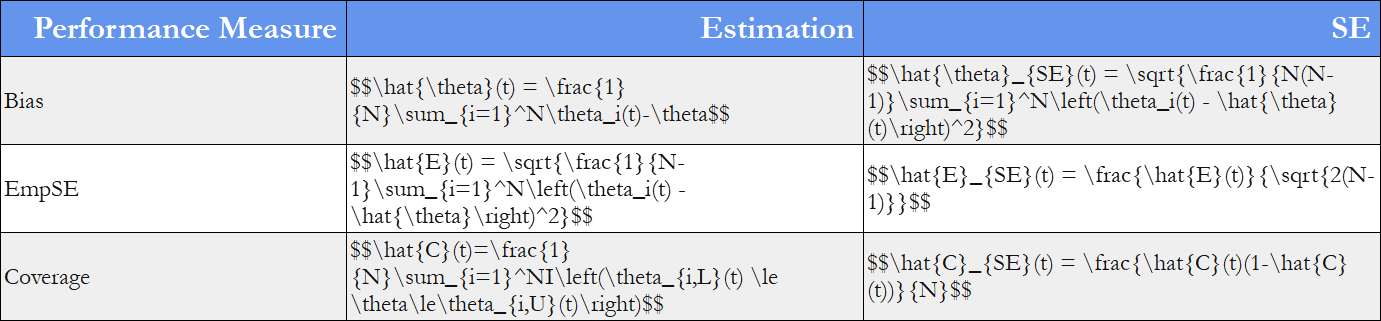
\includegraphics[width=6.30in,height=0.84in,keepaspectratio]{thesis_files/figure-latex/PM-DGM-time-1.png}

\label{tab:PM-DGM-time} Description of the Performance Measures defined at time \(t\)

For each estimand above, \(\hat{Q}(t) = \{\hat{\theta}(t),\hat{E}(t), \hat{C}(t)\}\) and associated SE, \(\hat{Q}_\textrm{SE}(t) = \{\hat{\theta}_\textrm{SE}(t),\hat{E}_\textrm{SE}(t), \hat{C}_\textrm{SE}(t)\}\), we average over time. As these measures will be taken at each of the 100 time points, \(t_j:j=1...100\), we summarise each of these measures as an average and as weighted average, as seen in table \ref{tab:PM-DGM}. The weight used for the measure at time \(t_j\) is the average number of non-censored patients remaining in the population at time \(t_j\), defined as \(n_j\) (note that this includes patients who have had the event).

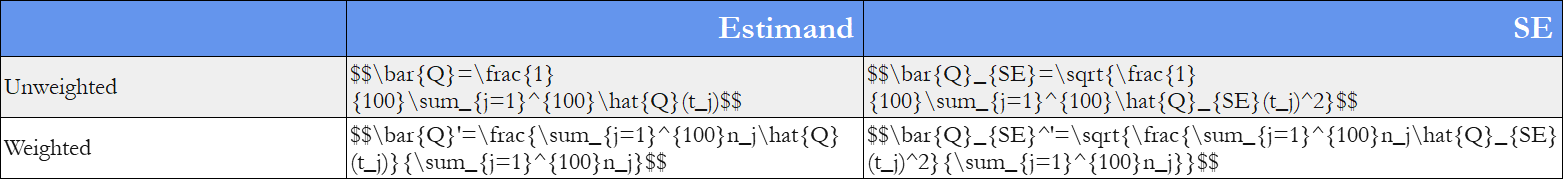
\includegraphics[width=6.30in,height=0.64in,keepaspectratio]{thesis_files/figure-latex/PM-DGM-1.png}

\label{tab:PM-DGM} Description of how Performance Measures are averaged over time

\hypertarget{software}{%
\subsection{Software}\label{software}}

All analysis was done in \texttt{R\ 3.6.3} {[}31{]} using the various \texttt{tidyverse} packages {[}32{]}, Kaplan-Meier estimates were found using the \texttt{survival} package {[}33{]}, Pseudo-Observations were evaluated with the \texttt{pseudo} package {[}34{]}.

\hypertarget{results}{%
\section{Results}\label{results}}

Forthcoming

\hypertarget{discussion}{%
\section{Discussion}\label{discussion}}

Weighting = Good.

Not Weighting = Bad.

\hypertarget{references}{%
\section{References}\label{references}}

\hypertarget{supplementary-material---calibration-slope}{%
\section{Supplementary Material - Calibration Slope}\label{supplementary-material---calibration-slope}}

The main purpose of this paper was to assess the evaluation of calibration-in-the-large at different time points in a time-to-event clinical prediction model. Along with calibration-in-the-large, various methods of calibration can also produce measures of calibration slope. Calibration slope provides an insight into how well the model predicts outcomes across the range of predictions. In an ideal model, the calibration slope would be 1. The Logistic Weighted, Logistic Unweighted and Pseudo-Observation methods described above can provide estimates of the calibration slope. For each of these methods, we first estimate the calibration-in-the-large as above, using a predictor as an offset, then we use this estimate as an offset to predict the calibration slope (without an intercept term).

\hypertarget{results-1}{%
\subsection{Results}\label{results-1}}

blah blah

\hypertarget{discussion-1}{%
\subsection{Discussion}\label{discussion-1}}

Brief discussion, much briefer than the main points.

\hypertarget{chap-performance-metrics}{%
\chapter{Prediction Model Performance Metrics for the Validation of Multi-State Clinical Prediction Models}\label{chap-performance-metrics}}

\hypertarget{introduction-3}{%
\section{Introduction}\label{introduction-3}}

Clinical Prediction Models (CPMs) provide individualised risk of a patient's outcome (cite), based on that patient's predictors. These predictions will usually be in the form of a risk score or probability. However, using traditional modelling techniques, these CPMs will only predict a single outcome. Multi-State Clinical Prediction Models (MS-CPMs) combine the multi-state modelling framework to the prognostic field to provide predictions for multiple outcomes in a single model.
Once a CPM has been developed, it is important to assess how well the model actually performs (cite). This process is called Model Validation and involves comparing the predictions produced by the model to the actual outcomes experienced by patients (cite). It is expected that the development of a CPM will be accompanied by the validation of the model on the same dataset it was developed in (internal validation), using either bootstrapping or cross-validation to account for optimism in the developed model (cite). Models can also be validated on a novel dataset (external validation), which is used to assess the generalisability and transportability of the model (cite).
During validation, there are different aspects of model performance that we can assess and these are measured using specific metrics. For example, to assess the overall Accuracy of a model, we may use the Brier Score (cite) or to analyse how well a model discriminates between patients, we could use the c-statistic (cite). The current metrics that are commonly used have been designed and extended to work in a variety of model development frameworks. However, these extensions are limited to either a single outcome (as in traditionally developed models) or do not adequately account for the censoring of patients (as commonly occurs in longitudinal data).
This paper aims to provide use-able extensions to current performance metrics to be used when validating MS-CPMs. It is essential that these extensions are directly comparable with current metrics (to allow for quicker adoption), that they are collapsible to the current metrics and that they adjust for the bias induced by the censoring of patients.
Currently, the most common way to validate an MS-CPMs is by applying traditional methods to compare across two states at a given time and then aggregating the results in an arbitrary manner {[}cite something{]}. Other methodologists have extended existing metrics to multinomial outcomes {[}cite van Calster{]}, which do not contain a time-based component; to simple competing risks scenarios {[}cite CR c-statistic{]}, which do not contain transient states; or to {[}\ldots{} insert third relevant example{]}. Spitoni et al {[}cite Spitoni 2018{]}{]} developed methods to apply the Brier Score (or any proper score functions) to a multi-state setting and so a simplified and specific version of their work is described in this paper.
It is the hope of the authors that this work will increase the uptake of multi-state models and the sub-field of MS-CPMs will grow appropriately.

\hypertarget{motivating-data-set}{%
\section{Motivating Data Set}\label{motivating-data-set}}

{[}\textbf{Table One for The Glasgow Data}{]}

Throughout this paper we will use a model developed in Chronic Kidney Disease (CKD) patients to assess their progression onto Renal Replacement Therapy (RRT) and/or Death {[}cite Dev/Valid Paper{]}. The model was developed using data from the Salford Kidney Study (SKS) and then applied to an external dataset derived from the West of Scotland (see Table 2) {[}1{]}. The original model predicts the probability that a patient has begun RRT and/or died after their first recorded eGFR below 60 ml/min/1.73m2, by any time in the future (reliable up to 10 years). For the purposes of this paper, we will take a ``snapshot'' of the predictions at the 5 year time point.
The Three-State model used in our example is designed as an Illness-Death Model {[}2{]}, this is one of the simplest MSM designs and has the key advantage over a traditional model that they can predict whether a patient is in or has visited the transient state before reaching the absorbing state (i.e.~patient who became ill before dying or who started RRT before dying) (see figure 1).

{[}\textbf{Figure of the MSM}{]}

{[}\textbf{Describe Glasgow Data}{]}

\hypertarget{current-approaches}{%
\section{Current Approaches}\label{current-approaches}}

Here we describe three commonly used performance metrics for assessing the performance of a traditional survival clinical prediction model. These metrics assess the Accuracy, Discrimination and Calibration of the models being validated. Accuracy is an overall measurement of how well the model predicts the outcomes in the patients. Discrimination assesses how well the model discerns between patients; in a two-state model this is a comparison of patients with and without the outcome, and should assign a higher value to those that experience the outcome. Calibration is the agreement between the observed outcomes and the predicted risks across the full risk-range.
We are applying cross-sectional metrics at a set time point within the setting of a longitudinal model and so we need to account for the censoring of patients and therefore, each uncensored patient at a given time t will be weighted as per the Inverse Probability of Censoring Weighting (IPCW) {[}3{]}. This allows the uncensored patient population to be representative of the entire patient population.

\hypertarget{baseline-models}{%
\subsection{Baseline Models}\label{baseline-models}}

To assess the performance of a model, we must compare the values produced by the performance metrics to those of two baseline models; a random or noninformative model and a perfect model.
A Non-Informative (NI-)model assigns the same probability to all patients to be in any state regardless of covariates and is akin to using the average prevalence in the entire population to define your model. For example, in a Two-State model and an event that occurs in 10\% of patients, all patients are predicted to have a 10\% chance of having the event. For many metrics, models can be compared to a Non-Informative model to assess whether the model is in fact ``better than random''.
A Perfect (P-)model is one which successfully assigns a 100\% probability to all patients, and the predictions are correct; this is the ideal case, which many models can also be compared to as models as close to this display excellent predictive abilities. Although models may perform worse than a non-informative one, we will not consider these in detail here as they are considered to be without worth in terms of predictive ability.
The metrics produced by these baseline models will often depend on the prevalence of each state and/or the number of states. These values can be used as comparators to provide contextual information regarding the strength of model performance. These baselines metrics for the NI-model and the P-model will be referred to as the NI-level and P-level for the metric.
In order to allow for simplicity and understanding of these measures, they will be standardised to the same scales.

\hypertarget{notation}{%
\subsection{Notation}\label{notation}}

Throughout this paper, we will use consistent notation which is shown here for reference and to avoid repetition in definitions, etc\ldots{}

{[}\textbf{Notation Table}{]}

\hypertarget{patient-weighting}{%
\subsection{Patient Weighting}\label{patient-weighting}}

{[}\textbf{Lots of formula, so will leave for now}{]}

\hypertarget{accuracy---brier-score}{%
\subsection{Accuracy - Brier Score}\label{accuracy---brier-score}}

\hypertarget{discrimination---c-statistic}{%
\subsection{Discrimination - c-statistic}\label{discrimination---c-statistic}}

\hypertarget{calibration---intercept-and-slope}{%
\subsection{Calibration - Intercept and Slope}\label{calibration---intercept-and-slope}}

\hypertarget{extension-to-multi-state-models}{%
\section{Extension to Multi-State Models}\label{extension-to-multi-state-models}}

\hypertarget{trivial-extensions}{%
\subsection{Trivial Extensions}\label{trivial-extensions}}

\hypertarget{accuracy---multiple-outcome-brier-score}{%
\subsection{Accuracy - Multiple Outcome Brier Score}\label{accuracy---multiple-outcome-brier-score}}

\hypertarget{discrimination---polytomous-discriminatory-index}{%
\subsection{Discrimination - Polytomous Discriminatory Index}\label{discrimination---polytomous-discriminatory-index}}

\hypertarget{computational-limitations}{%
\subsubsection{Computational Limitations}\label{computational-limitations}}

\hypertarget{calibration---multinomial-intercept-matched-and-unmatched-slopes}{%
\subsection{Calibration - Multinomial Intercept, Matched and Unmatched Slopes}\label{calibration---multinomial-intercept-matched-and-unmatched-slopes}}

\hypertarget{application-to-real-world-data}{%
\section{Application to Real-World Data}\label{application-to-real-world-data}}

\hypertarget{accuracy}{%
\subsection{Accuracy}\label{accuracy}}

\hypertarget{discrimination}{%
\subsection{Discrimination}\label{discrimination}}

\hypertarget{calibration}{%
\subsection{Calibration}\label{calibration}}

\hypertarget{discussion-2}{%
\section{Discussion}\label{discussion-2}}

\hypertarget{chap-dev-paper}{%
\chapter{Development and External Validation of a Multi-State Clinical Prediction Model for Chronic Kidney Disease Patients Progressing onto Renal Replacement Therapy and Death}\label{chap-dev-paper}}

\hypertarget{introduction-4}{%
\section{Introduction}\label{introduction-4}}

A testing \sout{introduction} beginning of a troubling time provides unsustainability.

What if I need to add a lot of text in between. Like an entirely new paragraph and it waffles on for a while until eventually it stops, but not before pushing the next paragraph further and further form down. This would move the old anchor point further and it's origin within the document. The risk is that it is only using the single word ``provides'' to find it. If it is, then there could be a problem when the test is expanded there are other copies of provides within othe regions which may be closer to the original. Alternatively, maybe it is using the surrounding phrase such as which provides or even provides patients, or both with a phrase like which provides patients.

A clinical prediction model (CPM) is a tool which provides patients and clinicians with a measure of how likely a patient is to suffer a specific clinical condition, more specifically, a prognostic model allows the prediction of future events {[}8{]}. CPMs use data from previous patients to estimate the outcomes of an individual patient. Prognostic models are used in clinical practice to influence treatment decisions such as the prescribing of statins for cardiovascular disease via the application of the QRISK models {[}2{]}.

Within Chronic Kidney Disease (CKD), prognostic models have been developed to predict mortality {[}35{]}--{[}39{]}, ESRD {[}36{]}, the commencements of RRT {[}38{]}, {[}40{]}--{[}42{]} or mortality after beginning dialysis {[}43{]}--{[}45{]}. Some previous models have used the commencement of RRT as a proxy for ESRD {[}46{]}--{[}48{]}, while others have investigated the occurrence of cardiovascular events within CKD patients{[}49{]}--{[}51{]}. Reviews by Grams \& Coresh {[}52{]}, Tangri et al {[}53{]} and Ramspek et al {[}54{]}, which explored the different aspects of assessing risk amongst CKD or RRT patients, found that the current landscape of CKD prediction models is lacking from both a methodological and clinical perspective {[}13{]}, {[}55{]}.

Methodologically, the majority of existing CKD prediction models fail to account for completing events {[}37{]}, {[}39{]}, {[}56{]}, have high risks of bias {[}35{]}, {[}36{]}, {[}40{]} or are otherwise flawed compared to modern clinical prediction standards {[}8{]}, {[}13{]}

In 2013, Begun et al {[}57{]} developed a multi-State model for assessing population-level progression through the severity stages of CKD (III-V), RRT and/or death, which can be used to provide a broad statement regarding a patient's future. In 2014, Allen et al {[}58{]} applied a similar model to liver transplant recipients and their progression through the stages of CKD with a focus on the predictions of measured vs estimated glomerular filtration rate (mGFR vs eGFR). In 2017, Kulkarni et al {[}42{]} developed an MSM focusing on the categories of Calculated Panel Reactive Antibodies (CPRA) and kidney transplant and/or death.

Most recently, in 2018, Grams et al {[}59{]} developed a multinomial clinical prediction model for CKD patients which focused on the occurrence of RRT and/or cardiovascular events. As of the publication of this paper, this is the only currently existing CPMs of this kind for CKD patients.

However, the first three of these existing models (Begun, Allen and Kulkarni) categorise continuous variables to define their states at specific cut-offs and this has been shown to be inefficient when modelling {[}60{]}--{[}78{]}. These kinds of cut-offs can be useful when informing patients and clinicians of a patient's diagnosis and to coincide with policy, but inherently cause a loss of information when done before the data analysis stage and so these models go against current statistical recommendations {[}60{]}--{[}78{]}. These kinds of assumptions are also subject to measurement error {[}79{]} and interval censoring {[}80{]}, i.e.~we do not know when exactly when a patient moved from CKD Stage III to CKD Stage IV, or whether drop in estimated Glomerular Function Rate (eGFR) was temporary or inaccurate. For example, Kulkarni {[}42{]} assumes that a patient with an CPRA of (5\%) is the same as a patient with an CPRA of (75\%) and that a patient with an CPRA of (89.9\%) is vastly different from a patient with an CPRA of (90\%). Moreover, none of these models have undergone any validation process, whether internal or external {[}10{]}.

It is also important to note that although these models can be used to predict patient outcomes, they were not designed to produce individualised patient predictions as is a key aspect of a clinical prediction model; they were designed to assess the methodological advantages of MSMs in this medical field, to describe the prevalence of over time of different CKD stages and to produce population level predictions for patients with different levels of panel-reactive antibodies {[}9{]}.

The fourth model (Grams), is presented as a Multi-State Model and the transitions involved were studied and defined, however the underlying statistical model is a pair of multinomial logistic models analysed at 2 and 4 years. The major downside of this model is that it can only produce predictions at those predefined time points and it assumes homogeneity of transition times. For example, the first model assumes that a patient who began RRT 1 month after study entry is the same as one who began after 1 year \& 11 months into the study and then the second model assumes these patients are the same as one who begins RRT at 3 years and 11 months.

Therefore, the aim of this study was to improve on previous efforts to model a patient's pathways through a Multi-State Model by choosing transition points which can be exactly identified and include states which produce a drastic difference in patient characteristics. Our modeling techniques allow for individual predictions (using a proportional hazards model) of multiple outcomes (using MSMs) at any time point (using cubic splines). The models produced by this process will then be validated, both internally and externally, to compare their results and demonstrate the transportability of the (statistically robust) clinical prediction models. We report our work in line with the TRIPOD guidelines for development and validation of clinical prediction models {[}13{]}, {[}14{]}.

\hypertarget{methods-4}{%
\section{Methods}\label{methods-4}}

\hypertarget{data-sources}{%
\subsection{Data Sources}\label{data-sources}}

The models were developed using data from the Salford Kidney Study (SKS) cohort of patients (previously named the CRISIS cohort), established in the Department of Renal Medicine, Salford Royal NHS Foundation Trust (SRFT). The SKS is a large longitudinal CKD cohort recruiting CKD patients since 2002. This cohort collects detailed annualised phenotypic and laboratory data, and plasma, serum and whole blood stored at -80\textdegree C for biomarker and genotypic analyses. Recruitment of patients into SKS has been described in multiple previous studies {[}81{]}, {[}82{]} and these have included a CKD progression prognostic factor study and to evidence the increased risk of cardiovascular events in diabetic kidney patients. In brief, any patient referred to Salford renal service (catchment population 1.5 million) who is 18 years or over and has an eGFR measurement of less than \(60\textrm{ml}/\textrm{min}/1.73\textrm{m}^2\) (calculated using the CKD-EPI formula {[}83{]}) was approached to be consented for the study participation.

At baseline, the data, including demographics, comorbidities, physical parameters, lab results and primary renal diagnosis are recorded in the database. Patients undergo an annual study visit and any changes to these parameters are captured. All data except blood results are collected via questionnaire by a dedicated team of research nurses. Blood results (baseline and annualised), first RRT modality and mortality outcome data are directly transferred to the database from Salford's Integrated Record (SIR) {[}84{]}. eGFR, uPCR, comorbidity and blood results were measured longitudinally throughout a patient's time within the cohort.

Due to limitations in our data, we were agnostic to how long since patients were diagnosed with CKD. Therefore, we defined a patient's start date for our model as their first date after consent at which their eGFR was recorded to be below \(60\textrm{ml}/\textrm{min}/1.73\textrm{m}^2\). Some patients consented with an eGFR that was already below 60, and some entered our study later when their eGFR was measured to be below 60. This implies that our models includes both patient who have recently been diagnosed with CKD (\(\textrm{eGFR} \lessapprox 60\)) \emph{and} those that have been suffering with CKD for an arbitrary amount of time. This timelessness of the model means it can be applied to any patient at any time during their CKD journey.

This allows for a wider range of baseline eGFR measurements and patients who have been suffering from CKD, translating to a model which can be applied to

All patients registered in the database between October 2002 and December 2016 with available data were included in this study. As this is a retrospective convenience sample, no sample size calculations were performed prior to recruitment. All patients were followed-up within SKS until the end-points of RRT, death or loss to follow-up or were censored at their last interaction with the healthcare system prior to December 2017. Date of death for patients who commenced RRT was also available within SIR and so also included in the SKS database.

For external validation of the model, we extracted an independent cohort from the West of Scotland Electronic Renal Patient Record (SERPR). Our extract of SERPR contains all patients known to the Glasgow and Forth Valley renal service who had an eGFR measure of less than \(60\textrm{ml}/\textrm{min}/1.73m^2\) between January 2006 and January 2016. This cohort has been previously used in Chronic Kidney Disease Prognosis consortium studies investigating outcomes in patients with CKD {[}85{]} and a similar cohort has been used for the analysis of skin tumours amongst renal transplant patients. Use of anonymised data from this database has been approved by the West of Scotland Ethics Committee for use of NHS Greater Glasgow and Clyde `Safe Haven' data for research.

Both the internal and external validation cohort were used as part of the multinational validation cohort used by Grams et al in their multinomial CPM discussed above {[}59{]}. In SERPR, start dates were calculated to be the first time point where the following conditions were met:
\begin{itemize}
\tightlist
\item
  eGFR is measured at less than 60
\item
  There is at least one prior eGFR measurement
\item
  Patient is 18 or over
\item
  Patient is not enduring an AKI {[}86{]}, {[}87{]}.
\end{itemize}
The second requirement was implemented to avoid a bias in the eGFR Rate. eGFR Rate is a measure of the change in eGFR over time and is calculated as the difference between the most recent two eGFR measurements divided by the time between them. For patients who entered the system with an \(\textrm{eGFR} < 60\), their eGFR Rate would be unavailable (i.e.~missing). Otherwise, patient eGFRs would \emph{have} to drop to below 60 and thus eGFR Rate would be negative. {[}\textbf{I feel like this bias should have a name, but can't think what to search to find it}{]}

\hypertarget{example}{%
\subsection{Example}\label{example}}

Once the models have been developed, we will apply them to two example patients to demonstrate their use and applicability to the general population. We will provide a direct clinical estimation of these patient outcomes based on years of nephrological experience and compare this with the results presented by our clinical prediction model.

We have chosen three (synthetic) patients to use as examples of the use of our model. Their details can be seen in table \ref{tab:Example-Patient}.
\begin{Shaded}
\begin{Highlighting}[]
\KeywordTok{tibble}\NormalTok{(}\DataTypeTok{id =} \DecValTok{1}\OperatorTok{:}\DecValTok{3}\NormalTok{,}\DataTypeTok{Age=}\KeywordTok{c}\NormalTok{(}\StringTok{"20"}\NormalTok{,}\StringTok{"40"}\NormalTok{,}\StringTok{"66"}\NormalTok{),}\DataTypeTok{Gender=}\KeywordTok{c}\NormalTok{(}\StringTok{"Female"}\NormalTok{,}\StringTok{"Male"}\NormalTok{,}\StringTok{"Female"}\NormalTok{),}
       \StringTok{\textasciigrave{}}\DataTypeTok{Smoking Status}\StringTok{\textasciigrave{}}\NormalTok{=}\KeywordTok{c}\NormalTok{(}\StringTok{"Non{-}Smoker"}\NormalTok{,}\StringTok{"Smoker"}\NormalTok{,}\StringTok{"Non{-}Smoker"}\NormalTok{),}
       \DataTypeTok{BP=}\KeywordTok{c}\NormalTok{(}\StringTok{"144/101"}\NormalTok{,}\StringTok{"160/90"}\NormalTok{,}\StringTok{"140/80"}\NormalTok{),}
       \DataTypeTok{Albumin=}\KeywordTok{c}\NormalTok{(}\StringTok{"39"}\NormalTok{,}\StringTok{"40"}\NormalTok{,}\StringTok{"40"}\NormalTok{),}\StringTok{\textasciigrave{}}\DataTypeTok{Correct Calcium}\StringTok{\textasciigrave{}}\NormalTok{=}\KeywordTok{c}\NormalTok{(}\StringTok{"2.3"}\NormalTok{,}\StringTok{"3.0"}\NormalTok{,}\StringTok{"2.6"}\NormalTok{),}
       \DataTypeTok{Haemoglobin=}\KeywordTok{c}\NormalTok{(}\StringTok{"150"}\NormalTok{,}\StringTok{"100"}\NormalTok{,}\StringTok{" 14"}\NormalTok{), }\DataTypeTok{Phosphate=}\KeywordTok{c}\NormalTok{(}\StringTok{"0.68"}\NormalTok{,}\StringTok{"2.00"}\NormalTok{,}\StringTok{"0.86"}\NormalTok{),}
       \DataTypeTok{eGFR=}\KeywordTok{c}\NormalTok{(}\StringTok{"42"}\NormalTok{,}\StringTok{"10"}\NormalTok{,}\StringTok{"51"}\NormalTok{),}
       \StringTok{\textasciigrave{}}\DataTypeTok{eGFR Previous}\StringTok{\textasciigrave{}}\NormalTok{=}\KeywordTok{c}\NormalTok{(}\StringTok{"50 (one week ago)"}\NormalTok{,}\StringTok{"30 (one year ago)"}\NormalTok{,}\StringTok{"70 (one week ago)"}\NormalTok{),}
       \DataTypeTok{uPCR=}\KeywordTok{c}\NormalTok{(}\StringTok{"0.30"}\NormalTok{,}\StringTok{"0.20"}\NormalTok{,}\StringTok{"0.01"}\NormalTok{),}
       \StringTok{\textasciigrave{}}\DataTypeTok{uPCR Previous}\StringTok{\textasciigrave{}}\NormalTok{=}\KeywordTok{c}\NormalTok{(}\StringTok{"0.80 (one month ago)"}\NormalTok{,}\StringTok{"1.20 (one year ago)"}\NormalTok{,}\StringTok{"0.06 (one week ago)"}\NormalTok{),}
       \StringTok{\textasciigrave{}}\DataTypeTok{Primary Diagnosis}\StringTok{\textasciigrave{}}\NormalTok{=}\KeywordTok{c}\NormalTok{(}\StringTok{"Glomerulonephritis"}\NormalTok{,}\StringTok{"Tubular Necrosis"}\NormalTok{,}\StringTok{"Diabetes"}\NormalTok{),}
       \DataTypeTok{Comorbities=}\KeywordTok{c}\NormalTok{(}\StringTok{"Chronic Obstructive Pulmonary Disease}\CharTok{\textbackslash{}n}\StringTok{Liver Disease}\CharTok{\textbackslash{}n}\StringTok{Solid Tumour"}\NormalTok{,}\StringTok{""}\NormalTok{,}
                     \StringTok{"Diabetes}\CharTok{\textbackslash{}n}\StringTok{Chronic Obstructive Pulmonary Disease}\CharTok{\textbackslash{}n}\StringTok{Hypertension"}\NormalTok{)) }\OperatorTok{\%>\%}
\StringTok{  }\KeywordTok{pivot\_longer}\NormalTok{(}\OperatorTok{{-}}\NormalTok{id,}\DataTypeTok{names\_to=}\StringTok{"Vars"}\NormalTok{,}\DataTypeTok{values\_to=}\StringTok{"Vals"}\NormalTok{) }\OperatorTok{\%>\%}\StringTok{ }
\StringTok{  }\KeywordTok{pivot\_wider}\NormalTok{(}\DataTypeTok{names\_from=}\NormalTok{id,}\DataTypeTok{values\_from=}\NormalTok{Vals,}\DataTypeTok{names\_prefix=}\StringTok{"Patient "}\NormalTok{) }\OperatorTok{\%>\%}
\StringTok{  }\NormalTok{flextable }\OperatorTok{\%>\%}
\StringTok{  }\KeywordTok{stardard\_format\_table}\NormalTok{(}\DataTypeTok{widths=}\DecValTok{5}\NormalTok{) }\OperatorTok{\%>\%}
\StringTok{  }\KeywordTok{align}\NormalTok{(}\DataTypeTok{part=}\StringTok{"header"}\NormalTok{,}\DataTypeTok{align=}\StringTok{"center"}\NormalTok{) }\OperatorTok{\%>\%}
\StringTok{  }\KeywordTok{align}\NormalTok{(}\DataTypeTok{part=}\StringTok{"body"}\NormalTok{,}\DataTypeTok{align=}\StringTok{"right"}\NormalTok{) }\OperatorTok{\%>\%}
\StringTok{  }\KeywordTok{padding}\NormalTok{(}\DataTypeTok{part=}\StringTok{"body"}\NormalTok{,}\DataTypeTok{padding.left=}\DecValTok{3}\NormalTok{, }\DataTypeTok{padding.right=}\DecValTok{3}\NormalTok{)}
\end{Highlighting}
\end{Shaded}
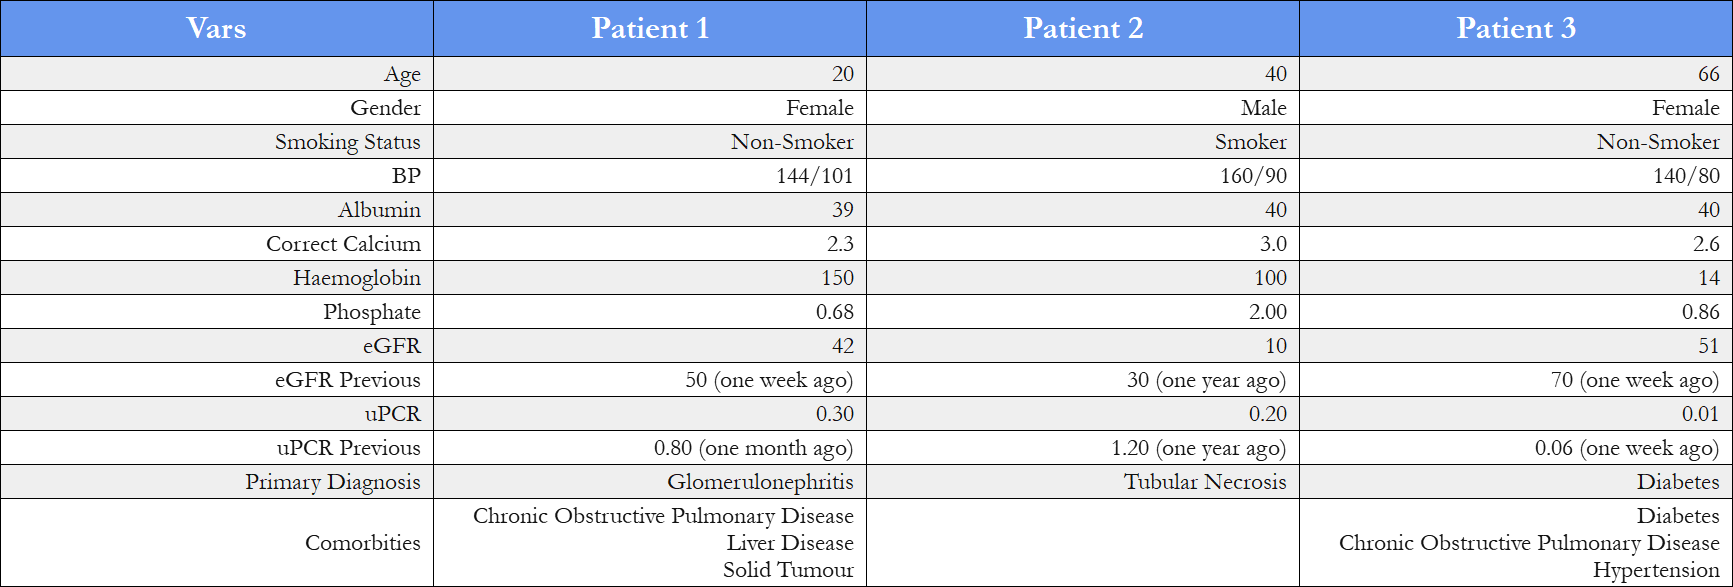
\includegraphics[width=7.87in,height=3.01in,keepaspectratio]{thesis_files/figure-latex/unnamed-chunk-1-1.png}
\begin{Shaded}
\begin{Highlighting}[]
\KeywordTok{add\_flextable\_caption}\NormalTok{(}\StringTok{"Example{-}Patient"}\NormalTok{,}\StringTok{"Details of the Example Patients"}\NormalTok{)}
\end{Highlighting}
\end{Shaded}
\begin{verbatim}
<caption>\label{tab:Example-Patient} Details of the Example Patients</caption>
\end{verbatim}
Out three example patients cover a broad range of ages and other covariates. A clinically guide prediction for these patients would assume that Patient 1 has a high chance of proceeding as normal (with little need for RRT), Patient 2 would be recommended to start RRT soon and Patient 3 would be predicted to have a high risk of mortality with or without RRT.

\hypertarget{calculator}{%
\subsection{Calculator}\label{calculator}}

As part of this work, we also intend to produce an online calculator to allow patients and clinicians to easily estimate outcomes without worrying about the mathematics involved.

All analysis was done in \texttt{R\ 3.6.2} {[}31{]} using the various \texttt{tidyverse} packages {[}32{]}, as well as the \texttt{mice} {[}88{]}, \texttt{flexsurv} {[}89{]}, \texttt{nnet} {[}90{]} and \texttt{furrr} {[}91{]} packages. The calculator was produced using the \texttt{shiny} package {[}92{]}.

\hypertarget{results-2}{%
\section{Results}\label{results-2}}

\hypertarget{data-sources-1}{%
\subsection{Data Sources}\label{data-sources-1}}

As seen in table \ref{tab:Continuous-Demo}, The Age of both populations were centred around 64-65 with a very broad range. Due to the inclusion criteria, eGFR were capped at a maximum of 60, and was consistent across populations; however, the rate of change for eGFR was much wider in the SERPR patients than in the SKS, and it was decreasing much faster, on average ( -25 vs 0) . Blood pressure was also consistent across populations (140/75 vs 148/76 for development vs validation). The blood test results (Corrected Calcium, Albumin, Haemoglobin and Phosphate) was close together, with the further difference being Haemoglobin with an average of 123 in SKS and 109 in SERPR and a much larger standard deviation in SERPR compared to SKS (38 vs 17). The uPCR measures are presented in our results as g/mmol, rather than the more conventional g/mol, this is to better present results and coefficients of varying magnitudes. Similar to the eGFR measures, the uPCR results were similar, but the rates of change were much broader in the validation dataset compared to the SKS and were generally increasing, whereas SKS remained stationary (73 vs 0). Levels of missingness were much higher in the SERPR dataset in most continuous variables.

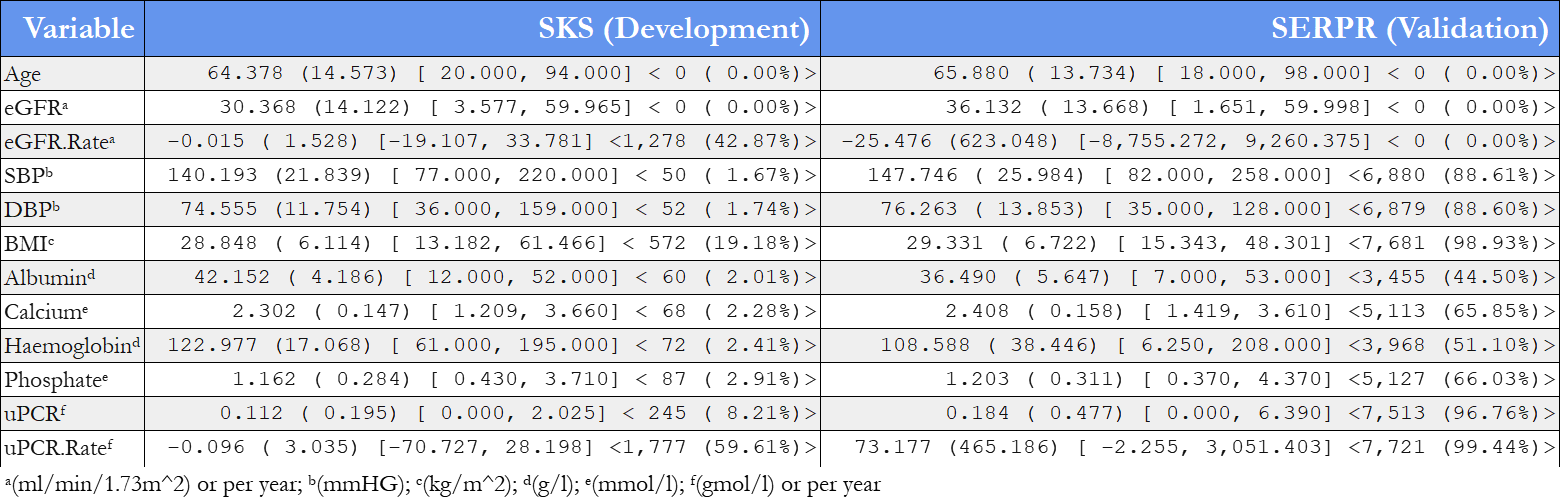
\includegraphics[width=7.23in,height=2.86in,keepaspectratio]{thesis_files/figure-latex/Continuous-Demo-1.png}

\label{tab:Continuous-Demo} Population demographics for the continuous variables presented as: mean (IQR) {[}min,max{]} \textless number missing (percent missing)\textgreater{}

Table \ref{tab:Categorical-Demo} shows a breakdown of the categorical variables across the populations. In the development population, there are far more males than females, whereas in the validation population the proportions are much more matched. Most patients were white in the SKS dataset, and ethnicity has extremely high missingness in SERPR, which also contributed to its omission from the model. The majority of the SKS patients were former smokers, however this information was unavailable in the SERPR dataset. Primary Renal Diagnosis suffered from very high levels of missingness in the validation dataset, but was much better recorded in the development dataset (although still far from perfect).

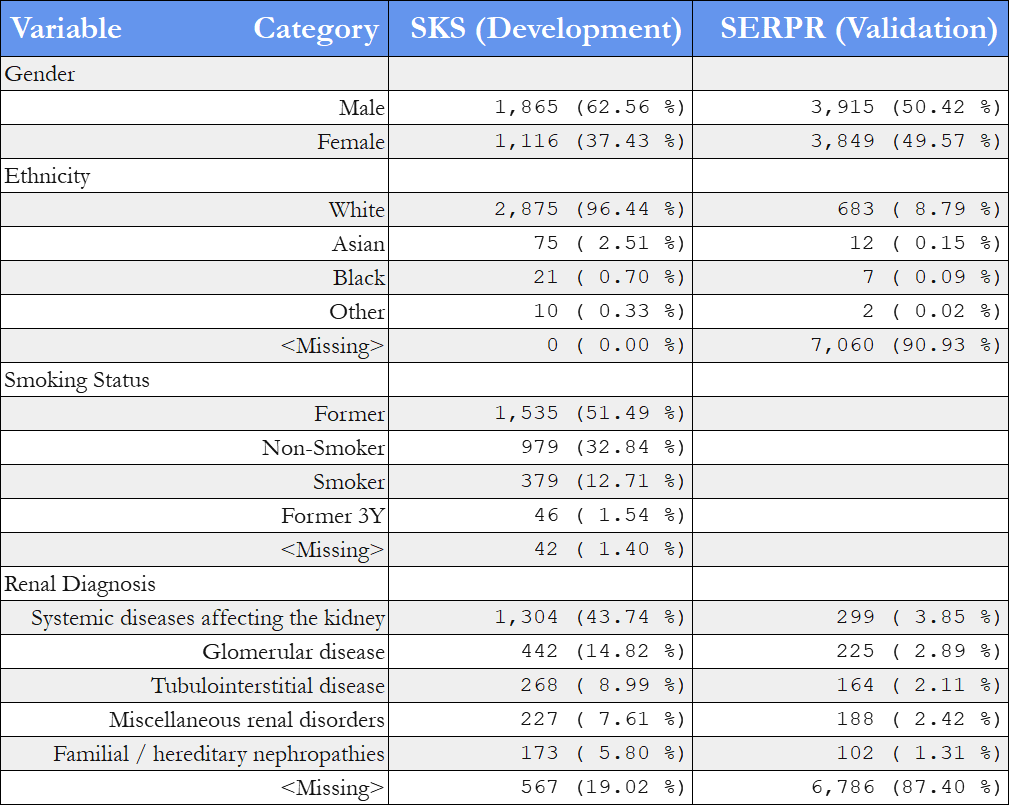
\includegraphics[width=4.53in,height=4.58in,keepaspectratio]{thesis_files/figure-latex/Categorical-Demo-1.png}

\label{tab:Categorical-Demo} Population demographics for the categorical variables presented as number (percent)

Overall, there were high levels of comorbidities within the SKS population as shown in table \ref{tab:Comorbidity-Demo}, but these levels were much lower in the SERPR population, possibly due to the data extraction processed (where data is un-recorded, no history is assumed). In SKS, most comorbidities were at over 80\% prevalence, apart from diabetes mellitus, which had a lower prevalence of 33\% and over 97\% (2,891) patients had a history of liver disease. In SERPR, hypertension was the highest prevalence in SERPR at 40\% (3,122), followed by diabetes mellitus at 20\% (1,546) and cerebrovascular accident was the lowest prevalence at 2.36\% (184). Liver disease, chronic obstructive pulmonary disease and solid tumour data were unavailable in the SERPR data.

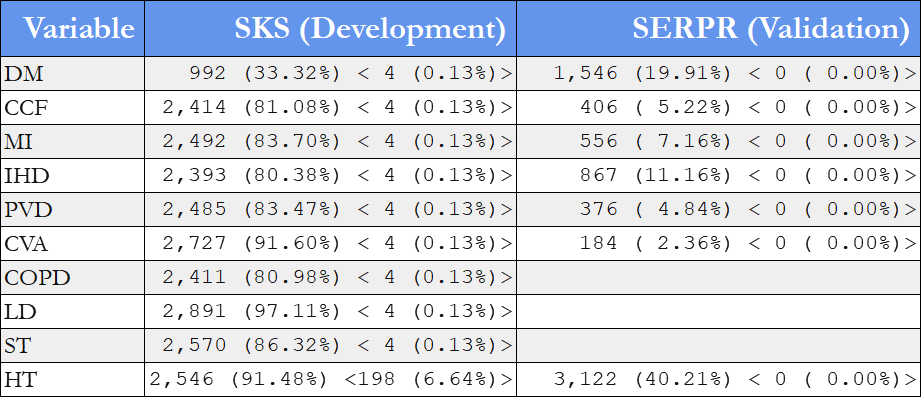
\includegraphics[width=4.26in,height=2.22in,keepaspectratio]{thesis_files/figure-latex/Comorbidity-Demo-1.png}

\label{tab:Comorbidity-Demo} Population comorbidity prevalence for the two populations presented as number (percent) \textless number missing (percent missing)\textgreater{}

The median date for the date of death was 3.9 years in the SKS population and 4.9 years in the SERPR population. The median date for transition to RRT was 2.2 years and 1.5 years (in SKS and SERPR respectively). In SKS, transitions to HD happened 6 months later than PD, and in SERPR it was 3.6 months. The Maximum followup time in SKS was 15.0 years and in SERPR it was 10.1 years. This information can be seen in table \ref{tab:Event-Median}.

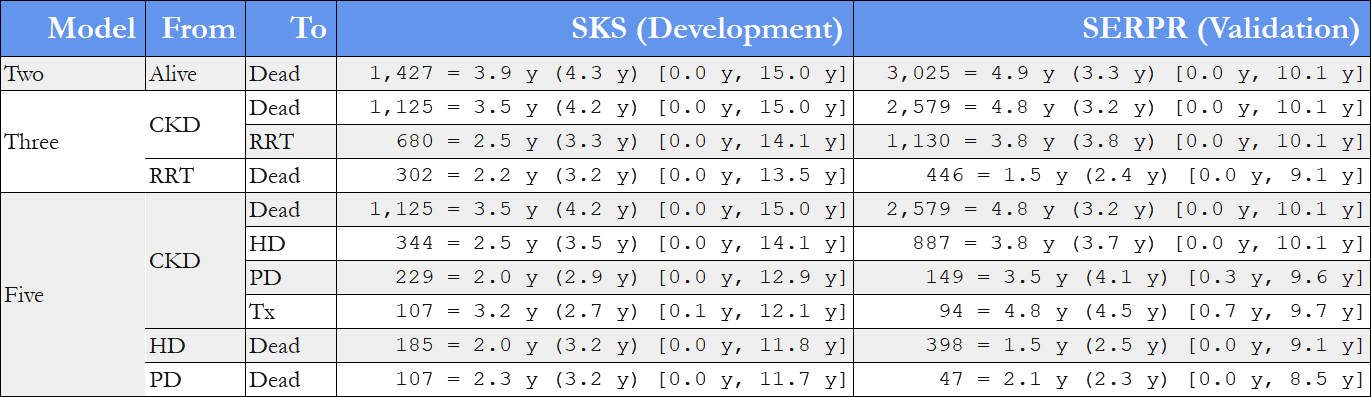
\includegraphics[width=6.20in,height=2.22in,keepaspectratio]{thesis_files/figure-latex/Event-Median-1.png}

\label{tab:Event-Median} Event times for the two populations presented as Number of Events = Median (Inter-Quartile Range) {[}Min, Max{]}

\hypertarget{example-1}{%
\subsection{Example}\label{example-1}}

The example patients seen in Table \ref{tab:Example-Patient} were passed through our Three-State prediction model and the results for all time-points are shown in figure \ref{fig:Example-Predictions-trend}. The prognosis for all three patients were very different. Patient 1 (20 year old) had a very high probability of survival, with only an 16\% chance of mortality by year 10 and 0\% chance of commencing RRT. Patient 2 (40 year old) was predicted almost 90\% chance of starting RRT, and over 70\% chance of dying overall (either with or without RR). Patient 3 (66 year old) had a fast acceleration towards high mortality, after 1 year from the recorded measurements, they had more than 50\% chance of dying, and after 2 years that probability rises to over 85\% with no chance of RRT.
\begin{figure}
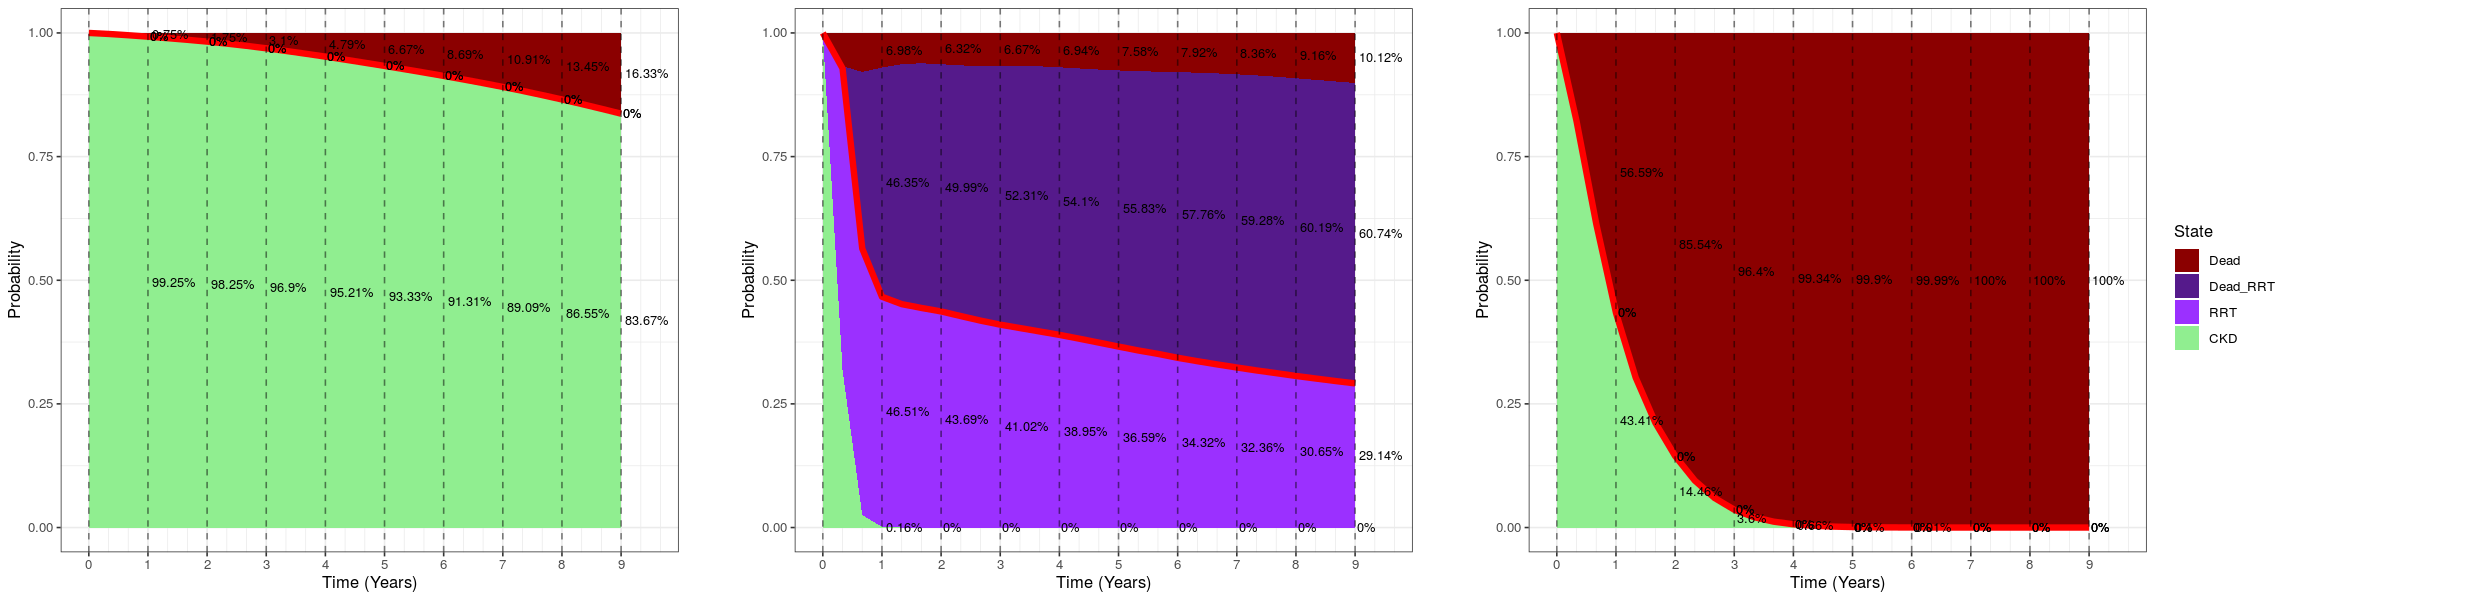
\includegraphics[width=34.29in]{figure/Dev_Paper_Example} \caption{Results of Example Patients}\label{fig:Example-Predictions-trend}
\end{figure}
\hypertarget{calculator-1}{%
\subsection{Calculator}\label{calculator-1}}

The calculator is available online here: \url{https://michael-barrowman.shinyapps.io/MSCPM_for_CKD_Patients/}.

\hypertarget{discussion-3}{%
\section{Discussion}\label{discussion-3}}

We have used data provided by SKS to develop a Multi-State Clinical Prediction Model and then validated this model within the SKS and SERPR datasets. Within our Models, the cause of a patient's renal disease had the widest effect on patient outcomes meaning that outcomes are highly dependent on ERA-EDTA classification of the diagnosis. Most groupings resulted in a lowered hazard of death and an increased hazard of RRT compared to the baseline of Systemic diseases.

Models performed well in model validation with the Three-State Model slightly out performing the other two models in calibration and overall predictive ability, however the Five-State model performed marginally better in terms of discriminative ability. Both Multi-State Models outperformed the Two-State (Traditional) Model.

The application of a Multi-state clinical prediction model to this field is novel and gives a powerful tool for providing individualised predictions of multiple outcomes at a wide range of time points. The general inclusion criteria for the development dataset, and the wide range of patient ages and measurements allows for the model to be applied to a broad spectrum of patients.

Although the inclusion criteria for SKS were broad, the demographics of the local area resulted in homogeneity of ethnicity, which may create a limitation to the applicability of our model. The Renal Department at SRFT is a tertiary care facility for CKD sufferers and is well renowned for its capabilities of care meaning that it is likely to attract less-healthy patients from a wider catchment area, making the cohort of patients in the development population in worse condition than the general population of CKD patients.

There were also high levels of missingness in the eGFR and uPCR rates of changes would also produce a bias, due to these measures likely being missing not at random. The derivation of the validation dataset ensured that all patients had an eGFR Rate measurement; this was done to avoid data missing not at random (only negative or missing data would be available as patient's eGFR dropped to less than 60), however deriving data in this way could itself induce a survivor bias in the start date used for patients.

In the Five-State Model, We omitted the analysis of the Tx to Dead state due to the anticipated low number of events within the SKS dataset. The lowest number of events for a transition was therefore PD to Dead, which had only 107. Altogether, we considered 26 covariates (with 4 categorical covariates) and so this equates to 36 predictor parameters and an events per predictor parameter (EPP) of 2.97. This is below the recommendations of Riley et al {[}93{]}, whose calculations produce a requirement of 4.54 EPP. This requirement was also not satisfied by the CKD to PD transition (EPP = 6.36,required = 10.2) or the CKD to Tx transition (EPP = 2.97, required = 17.6). Fortunately, this limitation is confined to the Five-State Model.

We have assumed a proportional hazards relationship between the predictors and probability of survival, which is considered by some to be a strong assumption to make, however we acknowledge this limitation, and the authors believe that it is mitigated by the flexibility that the assumption permits. In addition to the general PH assumption, the R-P model requires the assumption that the log cumulative hazard function follows a cubic spline, (however this is a much weaker assumption {[}94{]}), which is modelled as part of the regression. We did not assess the viability of these models as it was believed this assumption to make our results more understandable.

Compared to the raw internal validation, the model performance during the external validation was worse for all metrics. However, once adjusted for optimism, the results were much more cohesive which implies that the model is highly transportable to a new population without much alterations being required. Due to the differences in the healthcare systems of England and Scotland, it can be appreciated that despite the populations being similar, their care would be different enough to emphasise a larger difference between our populations than that shown in our (relatively homogeneous) populations.

Although not directly assessing causality in regards to state-transitions, our Three-State model can be used by clinicians to either expedite or delay transition of a patient onto RRT, if it is believed that this would be beneficial. Alternatively, the Five-State Model can be interpreted to provide information regarding \emph{which} treatment might be benficial for a patient.

Our paper has clearly demonstrated the accuracy of such a model. However, further research would be needed to establish the effectiveness and efficacy of its use in clinical practice {[}95{]} by comparing it to standard care and establishing whether the use of our model improves patient outcomes.

All three models produced for this work performed well in terms of accuracy, calibration and discrimination when applied internally and externally. This shows directly that the models are suitable for use in populations similar to both our development and our validation datasets. It can also be concluded that the models can be transported and applied to any population with a similar healthcare system to the UK.

\hypertarget{chap-conclusion}{%
\chapter{Conclusion}\label{chap-conclusion}}

Here is where my concluding section will go.

The final word.

The end.

\backmatter

\hypertarget{references-1}{%
\chapter*{References}\label{references-1}}
\addcontentsline{toc}{chapter}{References}

\markboth{References}{References}

\noindent

\setlength{\parindent}{-0.20in}
\setlength{\leftskip}{0.20in}
\setlength{\parskip}{8pt}

\hypertarget{refs}{}
\begin{cslreferences}
\leavevmode\hypertarget{ref-hippocrates_genuine_1886}{}%
{[}1{]} Hippocrates and F. Adams, \emph{The genuine works of Hippocrates;} New York, W. Wood and company, 1886.

\leavevmode\hypertarget{ref-hippisley-cox_development_2017}{}%
{[}2{]} J. Hippisley-Cox, C. Coupland, and P. Brindle, ``Development and validation of QRISK3 risk prediction algorithms to estimate future risk of cardiovascular disease: Prospective cohort study,'' \emph{BMJ}, vol. 357, May 2017, doi: \href{https://doi.org/10.1136/bmj.j2099}{10.1136/bmj.j2099}.

\leavevmode\hypertarget{ref-hemingway_prognosis_2013}{}%
{[}3{]} H. Hemingway \emph{et al.}, ``Prognosis research strategy (PROGRESS) 1: A framework for researching clinical outcomes,'' \emph{BMJ}, vol. 346, p. e5595, Feb. 2013, doi: \href{https://doi.org/10.1136/bmj.e5595}{10.1136/bmj.e5595}.

\leavevmode\hypertarget{ref-thygesen_universal_2007}{}%
{[}4{]} K. Thygesen, J. S. Alpert, H. D. White, and Joint ESC/ACCF/AHA/WHF Task Force for the Redefinition of Myocardial Infarction, ``Universal definition of myocardial infarction,'' \emph{Journal of the American College of Cardiology}, vol. 50, no. 22, pp. 2173--2195, Nov. 2007, doi: \href{https://doi.org/10.1016/j.jacc.2007.09.011}{10.1016/j.jacc.2007.09.011}.

\leavevmode\hypertarget{ref-probst_long-term_2010}{}%
{[}5{]} Probst \emph{et al.}, ``Long-Term Prognosis of Patients Diagnosed With Brugada Syndrome,'' \emph{Circulation}, vol. 121, no. 5, pp. 635--643, Feb. 2010, doi: \href{https://doi.org/10.1161/CIRCULATIONAHA.109.887026}{10.1161/CIRCULATIONAHA.109.887026}.

\leavevmode\hypertarget{ref-riley_prognosis_2019}{}%
{[}6{]} R. D. Riley, D. van der Windt, P. Croft, and K. G. M. Moons, \emph{Prognosis Research in Healthcare: Concepts, Methods, and Impact}, First. Oxford University Press, 2019.

\leavevmode\hypertarget{ref-riley_prognosis_2013}{}%
{[}7{]} R. D. Riley \emph{et al.}, ``Prognosis Research Strategy (PROGRESS) 2: Prognostic Factor Research,'' \emph{PLoS Medicine}, vol. 10, no. 2, Feb. 2013, doi: \href{https://doi.org/10.1371/journal.pmed.1001380}{10.1371/journal.pmed.1001380}.

\leavevmode\hypertarget{ref-steyerberg_prognosis_2013}{}%
{[}8{]} E. W. Steyerberg \emph{et al.}, ``Prognosis Research Strategy (PROGRESS) 3: Prognostic Model Research,'' \emph{PLOS Medicine}, vol. 10, no. 2, p. e1001381, Feb. 2013, doi: \href{https://doi.org/10.1371/journal.pmed.1001381}{10.1371/journal.pmed.1001381}.

\leavevmode\hypertarget{ref-royston_prognosis_2009}{}%
{[}9{]} P. Royston, K. G. M. Moons, D. G. Altman, and Y. Vergouwe, ``Prognosis and prognostic research: Developing a prognostic model,'' \emph{BMJ}, vol. 338, p. b604, Mar. 2009, doi: \href{https://doi.org/10.1136/bmj.b604}{10.1136/bmj.b604}.

\leavevmode\hypertarget{ref-altman_prognosis_2009}{}%
{[}10{]} D. G. Altman, Y. Vergouwe, P. Royston, and K. G. M. Moons, ``Prognosis and prognostic research: Validating a prognostic model,'' \emph{BMJ}, vol. 338, p. b605, May 2009, doi: \href{https://doi.org/10.1136/bmj.b605}{10.1136/bmj.b605}.

\leavevmode\hypertarget{ref-moons_prognosis_2009}{}%
{[}11{]} K. G. M. Moons, P. Royston, Y. Vergouwe, D. E. Grobbee, and D. G. Altman, ``Prognosis and prognostic research: What, why, and how?'' \emph{BMJ}, vol. 338, p. b375, Feb. 2009, doi: \href{https://doi.org/10.1136/bmj.b375}{10.1136/bmj.b375}.

\leavevmode\hypertarget{ref-hingorani_prognosis_2013}{}%
{[}12{]} A. D. Hingorani \emph{et al.}, ``Prognosis research strategy (PROGRESS) 4: Stratified medicine research,'' \emph{BMJ}, vol. 346, p. e5793, Feb. 2013, doi: \href{https://doi.org/10.1136/bmj.e5793}{10.1136/bmj.e5793}.

\leavevmode\hypertarget{ref-collins_transparent_2015}{}%
{[}13{]} G. S. Collins, J. B. Reitsma, D. G. Altman, and K. G. Moons, ``Transparent reporting of a multivariable prediction model for individual prognosis or diagnosis (TRIPOD): The TRIPOD Statement,'' \emph{BMC Medicine}, vol. 13, no. 1, p. 1, Jan. 2015, doi: \href{https://doi.org/10.1186/s12916-014-0241-z}{10.1186/s12916-014-0241-z}.

\leavevmode\hypertarget{ref-moons_transparent_2015}{}%
{[}14{]} K. G. M. Moons \emph{et al.}, ``Transparent Reporting of a multivariable prediction model for Individual Prognosis Or Diagnosis (TRIPOD): Explanation and Elaboration,'' \emph{Annals of Internal Medicine}, vol. 162, no. 1, p. W1, Jan. 2015, doi: \href{https://doi.org/10.7326/M14-0698}{10.7326/M14-0698}.

\leavevmode\hypertarget{ref-steyerberg_clinical_2008}{}%
{[}15{]} E. W. Steyerberg, \emph{Clinical Prediction Models: A Practical Approach to Development, Validation, and Updating}. Springer Science \& Business Media, 2008.

\leavevmode\hypertarget{ref-calster_calibration_2016-1}{}%
{[}16{]} B. V. Calster, D. Nieboer, Y. Vergouwe, B. D. Cock, M. J. Pencina, and E. W. Steyerberg, ``A calibration hierarchy for risk models was defined: From utopia to empirical data,'' \emph{Journal of Clinical Epidemiology}, vol. 74, pp. 167--176, Jun. 2016, doi: \href{https://doi.org/10.1016/j.jclinepi.2015.12.005}{10.1016/j.jclinepi.2015.12.005}.

\leavevmode\hypertarget{ref-royston_external_2013}{}%
{[}17{]} P. Royston and D. G. Altman, ``External validation of a Cox prognostic model: Principles and methods,'' \emph{BMC Medical Research Methodology}, vol. 13, no. 1, p. 33, Mar. 2013, doi: \href{https://doi.org/10.1186/1471-2288-13-33}{10.1186/1471-2288-13-33}.

\leavevmode\hypertarget{ref-crowson_assessing_2016}{}%
{[}18{]} C. S. Crowson, E. J. Atkinson, and T. M. Therneau, ``Assessing Calibration of Prognostic Risk Scores,'' \emph{Statistical methods in medical research}, vol. 25, no. 4, pp. 1692--1706, Aug. 2016, doi: \href{https://doi.org/10.1177/0962280213497434}{10.1177/0962280213497434}.

\leavevmode\hypertarget{ref-houwelingen_validation_2000}{}%
{[}19{]} H. C. van Houwelingen, ``Validation, calibration, revision and combination of prognostic survival models,'' \emph{Statistics in Medicine}, vol. 19, no. 24, pp. 3401--3415, 2000, doi: \href{https://doi.org/10.1002/1097-0258(20001230)19:24\%3C3401::AID-SIM554\%3E3.0.CO;2-2}{10.1002/1097-0258(20001230)19:24\textless3401::AID-SIM554\textgreater3.0.CO;2-2}.

\leavevmode\hypertarget{ref-hippisley-cox_derivation_2007}{}%
{[}20{]} J. Hippisley-Cox, C. Coupland, Y. Vinogradova, J. Robson, M. May, and P. Brindle, ``Derivation and validation of QRISK, a new cardiovascular disease risk score for the United Kingdom: Prospective open cohort study,'' \emph{BMJ (Clinical research ed.)}, vol. 335, no. 7611, p. 136, Jul. 2007, doi: \href{https://doi.org/10.1136/bmj.39261.471806.55}{10.1136/bmj.39261.471806.55}.

\leavevmode\hypertarget{ref-royston_tools_2014}{}%
{[}21{]} P. Royston, ``Tools for Checking Calibration of a Cox Model in External Validation: Approach Based on Individual Event Probabilities:'' \emph{The Stata Journal}, Dec. 2014, doi: \href{https://doi.org/10.1177/1536867X1401400403}{10.1177/1536867X1401400403}.

\leavevmode\hypertarget{ref-perme_checking_2008}{}%
{[}22{]} M. P. Perme and P. K. Andersen, ``Checking hazard regression models using pseudo-observations,'' \emph{Statistics in medicine}, vol. 27, no. 25, pp. 5309--5328, Nov. 2008, doi: \href{https://doi.org/10.1002/sim.3401}{10.1002/sim.3401}.

\leavevmode\hypertarget{ref-royston_tools_2015}{}%
{[}23{]} P. Royston, ``Tools for Checking Calibration of a Cox Model in External Validation: Prediction of Population-Averaged Survival Curves Based on Risk Groups,'' \emph{The Stata Journal}, vol. 15, no. 1, pp. 275--291, Apr. 2015, doi: \href{https://doi.org/10.1177/1536867X1501500116}{10.1177/1536867X1501500116}.

\leavevmode\hypertarget{ref-gerds_consistent_2006}{}%
{[}24{]} T. A. Gerds and M. Schumacher, ``Consistent Estimation of the Expected Brier Score in General Survival Models with Right-Censored Event Times,'' \emph{Biometrical Journal}, vol. 48, no. 6, pp. 1029--1040, 2006, doi: \href{https://doi.org/10.1002/bimj.200610301}{10.1002/bimj.200610301}.

\leavevmode\hypertarget{ref-spitoni_prediction_2018}{}%
{[}25{]} C. Spitoni, V. Lammens, and H. Putter, ``Prediction errors for state occupation and transition probabilities in multi-state models,'' \emph{Biometrical Journal. Biometrische Zeitschrift}, vol. 60, no. 1, pp. 34--48, Jan. 2018, doi: \href{https://doi.org/10.1002/bimj.201600191}{10.1002/bimj.201600191}.

\leavevmode\hypertarget{ref-han_comparing_2017}{}%
{[}26{]} X. Han, Y. Zhang, and Y. Shao, ``On comparing two correlated C indices with censored survival data,'' \emph{Statistics in medicine}, vol. 36, no. 25, pp. 4041--4049, Nov. 2017, doi: \href{https://doi.org/10.1002/sim.7414}{10.1002/sim.7414}.

\leavevmode\hypertarget{ref-liu_comparing_2016}{}%
{[}27{]} X. Liu, Z. Jin, and J. H. Graziano, ``Comparing paired biomarkers in predicting quantitative health outcome subject to random censoring,'' \emph{Statistical methods in medical research}, vol. 25, no. 1, pp. 447--457, Feb. 2016, doi: \href{https://doi.org/10.1177/0962280212460434}{10.1177/0962280212460434}.

\leavevmode\hypertarget{ref-burton_design_2006}{}%
{[}28{]} A. Burton, D. G. Altman, P. Royston, and R. L. Holder, ``The design of simulation studies in medical statistics,'' \emph{Statistics in Medicine}, vol. 25, no. 24, pp. 4279--4292, Dec. 2006, doi: \href{https://doi.org/10.1002/sim.2673}{10.1002/sim.2673}.

\leavevmode\hypertarget{ref-andersen_pseudo-observations_2010}{}%
{[}29{]} P. K. Andersen and M. Pohar Perme, ``Pseudo-observations in survival analysis,'' \emph{Statistical Methods in Medical Research}, vol. 19, no. 1, pp. 71--99, Feb. 2010, doi: \href{https://doi.org/10.1177/0962280209105020}{10.1177/0962280209105020}.

\leavevmode\hypertarget{ref-morris_using_2019}{}%
{[}30{]} T. P. Morris, I. R. White, and M. J. Crowther, ``Using simulation studies to evaluate statistical methods,'' \emph{Statistics in Medicine}, vol. 38, no. 11, pp. 2074--2102, 2019, doi: \href{https://doi.org/10.1002/sim.8086}{10.1002/sim.8086}.

\leavevmode\hypertarget{ref-r_core_team_r_nodate}{}%
{[}31{]} R. C. Team, ``R: A Language and Environment for Statistical Computing.'' R Foundation for Statistical Computing, Vienna, Austria, Vienna,

\leavevmode\hypertarget{ref-wickham_tidy_2017}{}%
{[}32{]} H. Wickham, ``The tidy tools manifesto.'' https://cran.r-project.org/web/packages/tidyverse/vignettes/manifesto.html, Nov-2017.

\leavevmode\hypertarget{ref-therneau_package_2020}{}%
{[}33{]} T. Therneau, ``A package for survival analysis in R,'' p. 89, Mar. 2020.

\leavevmode\hypertarget{ref-perme_pseudo_2017}{}%
{[}34{]} M. P. Perme, M. Gerster, and K. Rodrigues, ``Pseudo: Computes Pseudo-Observations for Modeling.'' Jul-2017.

\leavevmode\hypertarget{ref-johnson_predicting_2007}{}%
{[}35{]} E. S. Johnson, M. L. Thorp, X. Yang, O. L. Charansonney, and D. H. Smith, ``Predicting renal replacement therapy and mortality in CKD,'' \emph{American Journal of Kidney Diseases: The Official Journal of the National Kidney Foundation}, vol. 50, no. 4, pp. 559--565, Oct. 2007, doi: \href{https://doi.org/10.1053/j.ajkd.2007.07.006}{10.1053/j.ajkd.2007.07.006}.

\leavevmode\hypertarget{ref-landray_prediction_2010}{}%
{[}36{]} M. J. Landray \emph{et al.}, ``Prediction of ESRD and death among people with CKD: The Chronic Renal Impairment in Birmingham (CRIB) prospective cohort study,'' \emph{American Journal of Kidney Diseases: The Official Journal of the National Kidney Foundation}, vol. 56, no. 6, pp. 1082--1094, Dec. 2010, doi: \href{https://doi.org/10.1053/j.ajkd.2010.07.016}{10.1053/j.ajkd.2010.07.016}.

\leavevmode\hypertarget{ref-bansal_development_2015}{}%
{[}37{]} N. Bansal \emph{et al.}, ``Development and validation of a model to predict 5-year risk of death without ESRD among older adults with CKD,'' \emph{Clinical journal of the American Society of Nephrology: CJASN}, vol. 10, no. 3, pp. 363--371, Mar. 2015, doi: \href{https://doi.org/10.2215/CJN.04650514}{10.2215/CJN.04650514}.

\leavevmode\hypertarget{ref-marks_looking_2015}{}%
{[}38{]} A. Marks \emph{et al.}, ``Looking to the future: Predicting renal replacement outcomes in a large community cohort with chronic kidney disease,'' \emph{Nephrology, Dialysis, Transplantation: Official Publication of the European Dialysis and Transplant Association - European Renal Association}, vol. 30, no. 9, pp. 1507--1517, Sep. 2015, doi: \href{https://doi.org/10.1093/ndt/gfv089}{10.1093/ndt/gfv089}.

\leavevmode\hypertarget{ref-wick_clinical_2017}{}%
{[}39{]} J. P. Wick \emph{et al.}, ``A Clinical Risk Prediction Tool for 6-Month Mortality After Dialysis Initiation Among Older Adults,'' \emph{American Journal of Kidney Diseases: The Official Journal of the National Kidney Foundation}, vol. 69, no. 5, pp. 568--575, May 2017, doi: \href{https://doi.org/10.1053/j.ajkd.2016.08.035}{10.1053/j.ajkd.2016.08.035}.

\leavevmode\hypertarget{ref-johnson_predicting_2008}{}%
{[}40{]} E. S. Johnson, M. L. Thorp, R. W. Platt, and D. H. Smith, ``Predicting the risk of dialysis and transplant among patients with CKD: A retrospective cohort study,'' \emph{American Journal of Kidney Diseases: The Official Journal of the National Kidney Foundation}, vol. 52, no. 4, pp. 653--660, Oct. 2008, doi: \href{https://doi.org/10.1053/j.ajkd.2008.04.026}{10.1053/j.ajkd.2008.04.026}.

\leavevmode\hypertarget{ref-schroeder_predicting_2017}{}%
{[}41{]} E. B. Schroeder \emph{et al.}, ``Predicting 5-Year Risk of RRT in Stage 3 or 4 CKD: Development and External Validation,'' \emph{Clinical journal of the American Society of Nephrology: CJASN}, vol. 12, no. 1, pp. 87--94, Jun. 2017, doi: \href{https://doi.org/10.2215/CJN.01290216}{10.2215/CJN.01290216}.

\leavevmode\hypertarget{ref-kulkarni_transition_2017}{}%
{[}42{]} S. Kulkarni \emph{et al.}, ``Transition probabilities between changing sensitization levels, waitlist activity status and competing-risk kidney transplant outcomes using multi-state modeling,'' \emph{PLOS ONE}, vol. 12, no. 12, p. e0190277, Dec. 2017, doi: \href{https://doi.org/10.1371/journal.pone.0190277}{10.1371/journal.pone.0190277}.

\leavevmode\hypertarget{ref-floege_development_2015}{}%
{[}43{]} J. Floege \emph{et al.}, ``Development and validation of a predictive mortality risk score from a European hemodialysis cohort,'' \emph{Kidney International}, vol. 87, no. 5, pp. 996--1008, May 2015, doi: \href{https://doi.org/10.1038/ki.2014.419}{10.1038/ki.2014.419}.

\leavevmode\hypertarget{ref-hemke_survival_2013}{}%
{[}44{]} A. C. Hemke, M. B. Heemskerk, M. van Diepen, W. Weimar, F. W. Dekker, and A. J. Hoitsma, ``Survival prognosis after the start of a renal replacement therapy in the Netherlands: A retrospective cohort study,'' \emph{BMC Nephrology}, vol. 14, p. 258, Nov. 2013, doi: \href{https://doi.org/10.1186/1471-2369-14-258}{10.1186/1471-2369-14-258}.

\leavevmode\hypertarget{ref-cao_predicting_2015}{}%
{[}45{]} X.-Y. Cao \emph{et al.}, ``Predicting one-year mortality in peritoneal dialysis patients: An analysis of the China Peritoneal Dialysis Registry,'' \emph{International Journal of Medical Sciences}, vol. 12, no. 4, pp. 354--361, 2015, doi: \href{https://doi.org/10.7150/ijms.11694}{10.7150/ijms.11694}.

\leavevmode\hypertarget{ref-tangri_predictive_2011}{}%
{[}46{]} N. Tangri \emph{et al.}, ``A predictive model for progression of chronic kidney disease to kidney failure,'' \emph{JAMA}, vol. 305, no. 15, pp. 1553--1559, Apr. 2011, doi: \href{https://doi.org/10.1001/jama.2011.451}{10.1001/jama.2011.451}.

\leavevmode\hypertarget{ref-roy_statistical_2017}{}%
{[}47{]} J. Roy \emph{et al.}, ``Statistical Methods for Cohort Studies of CKD: Prediction Modeling,'' \emph{Clinical journal of the American Society of Nephrology: CJASN}, vol. 12, no. 6, pp. 1010--1017, Jun. 2017, doi: \href{https://doi.org/10.2215/CJN.06210616}{10.2215/CJN.06210616}.

\leavevmode\hypertarget{ref-tangri_dynamic_2017}{}%
{[}48{]} N. Tangri \emph{et al.}, ``A Dynamic Predictive Model for Progression of CKD,'' \emph{American Journal of Kidney Diseases: The Official Journal of the National Kidney Foundation}, vol. 69, no. 4, pp. 514--520, Apr. 2017, doi: \href{https://doi.org/10.1053/j.ajkd.2016.07.030}{10.1053/j.ajkd.2016.07.030}.

\leavevmode\hypertarget{ref-shlipak_cardiovascular_2005}{}%
{[}49{]} M. G. Shlipak \emph{et al.}, ``Cardiovascular mortality risk in chronic kidney disease: Comparison of traditional and novel risk factors,'' \emph{JAMA}, vol. 293, no. 14, pp. 1737--1745, Apr. 2005, doi: \href{https://doi.org/10.1001/jama.293.14.1737}{10.1001/jama.293.14.1737}.

\leavevmode\hypertarget{ref-weiner_framingham_2007}{}%
{[}50{]} D. E. Weiner \emph{et al.}, ``The Framingham predictive instrument in chronic kidney disease,'' \emph{Journal of the American College of Cardiology}, vol. 50, no. 3, pp. 217--224, Jul. 2007, doi: \href{https://doi.org/10.1016/j.jacc.2007.03.037}{10.1016/j.jacc.2007.03.037}.

\leavevmode\hypertarget{ref-mcmurray_predictors_2011}{}%
{[}51{]} J. J. V. McMurray \emph{et al.}, ``Predictors of fatal and nonfatal cardiovascular events in patients with type 2 diabetes mellitus, chronic kidney disease, and anemia: An analysis of the Trial to Reduce cardiovascular Events with Aranesp (darbepoetin-alfa) Therapy (TREAT),'' \emph{American Heart Journal}, vol. 162, no. 4, pp. 748--755.e3, Oct. 2011, doi: \href{https://doi.org/10.1016/j.ahj.2011.07.016}{10.1016/j.ahj.2011.07.016}.

\leavevmode\hypertarget{ref-grams_assessing_2013}{}%
{[}52{]} M. E. Grams and J. Coresh, ``Assessing risk in chronic kidney disease: A methodological review,'' \emph{Nature Reviews. Nephrology}, vol. 9, no. 1, pp. 18--25, Jan. 2013, doi: \href{https://doi.org/10.1038/nrneph.2012.248}{10.1038/nrneph.2012.248}.

\leavevmode\hypertarget{ref-tangri_risk_2013}{}%
{[}53{]} N. Tangri \emph{et al.}, ``Risk prediction models for patients with chronic kidney disease: A systematic review,'' \emph{Annals of Internal Medicine}, vol. 158, no. 8, pp. 596--603, Apr. 2013, doi: \href{https://doi.org/10.7326/0003-4819-158-8-201304160-00004}{10.7326/0003-4819-158-8-201304160-00004}.

\leavevmode\hypertarget{ref-ramspek_prediction_2017}{}%
{[}54{]} C. L. Ramspek, P. W. Voskamp, F. J. van Ittersum, R. T. Krediet, F. W. Dekker, and M. van Diepen, ``Prediction models for the mortality risk in chronic dialysis patients: A systematic review and independent external validation study,'' \emph{Clinical Epidemiology}, vol. 9, pp. 451--464, 2017, doi: \href{https://doi.org/10.2147/CLEP.S139748}{10.2147/CLEP.S139748}.

\leavevmode\hypertarget{ref-bouwmeester_reporting_2012-1}{}%
{[}55{]} W. Bouwmeester \emph{et al.}, ``Reporting and Methods in Clinical Prediction Research: A Systematic Review,'' \emph{PLOS Medicine}, vol. 9, no. 5, p. e1001221, May 2012, doi: \href{https://doi.org/10.1371/journal.pmed.1001221}{10.1371/journal.pmed.1001221}.

\leavevmode\hypertarget{ref-perotte_risk_2015}{}%
{[}56{]} A. Perotte, R. Ranganath, J. S. Hirsch, D. Blei, and N. Elhadad, ``Risk prediction for chronic kidney disease progression using heterogeneous electronic health record data and time series analysis,'' \emph{Journal of the American Medical Informatics Association: JAMIA}, vol. 22, no. 4, pp. 872--880, Jul. 2015, doi: \href{https://doi.org/10.1093/jamia/ocv024}{10.1093/jamia/ocv024}.

\leavevmode\hypertarget{ref-begun_identification_2013}{}%
{[}57{]} A. Begun, A. Icks, R. Waldeyer, S. Landwehr, M. Koch, and G. Giani, ``Identification of a multistate continuous-time nonhomogeneous Markov chain model for patients with decreased renal function.'' \emph{Medical decision making : an international journal of the Society for Medical Decision Making}, vol. 33, no. 2, pp. 298--306, Feb. 2013, doi: \href{https://doi.org/10.1177/0272989X12466731}{10.1177/0272989X12466731}.

\leavevmode\hypertarget{ref-allen_chronic_2014}{}%
{[}58{]} A. M. Allen, W. R. Kim, T. M. Therneau, J. J. Larson, J. K. Heimbach, and A. D. Rule, ``Chronic kidney disease and associated mortality after liver transplantation--a time-dependent analysis using measured glomerular filtration rate,'' \emph{Journal of Hepatology}, vol. 61, no. 2, pp. 286--292, Aug. 2014, doi: \href{https://doi.org/10.1016/j.jhep.2014.03.034}{10.1016/j.jhep.2014.03.034}.

\leavevmode\hypertarget{ref-grams_predicting_2018}{}%
{[}59{]} M. E. Grams \emph{et al.}, ``Predicting timing of clinical outcomes in patients~with chronic kidney disease and severely decreased glomerular filtration rate,'' \emph{Kidney International}, vol. 93, no. 6, pp. 1442--1451, Jun. 2018, doi: \href{https://doi.org/10.1016/j.kint.2018.01.009}{10.1016/j.kint.2018.01.009}.

\leavevmode\hypertarget{ref-altman_problems_1994-1}{}%
{[}60{]} D. G. Altman, ``Problems in dichotomizing continuous variables,'' \emph{American Journal of Epidemiology}, vol. 139, no. 4, pp. 442--445, Feb. 1994, doi: \href{https://doi.org/10.1093/oxfordjournals.aje.a117020}{10.1093/oxfordjournals.aje.a117020}.

\leavevmode\hypertarget{ref-altman_dangers_1994-1}{}%
{[}61{]} D. G. Altman, B. Lausen, W. Sauerbrei, and M. Schumacher, ``Dangers of Using `Optimal' Cutpoints in the Evaluation of Prognostic Factors,'' \emph{JNCI: Journal of the National Cancer Institute}, vol. 86, no. 11, pp. 829--835, Jun. 1994, doi: \href{https://doi.org/10.1093/jnci/86.11.829}{10.1093/jnci/86.11.829}.

\leavevmode\hypertarget{ref-altman_cost_2006-1}{}%
{[}62{]} D. G. Altman and P. Royston, ``The cost of dichotomising continuous variables,'' \emph{BMJ}, vol. 332, no. 7549, p. 1080, May 2006, doi: \href{https://doi.org/10.1136/bmj.332.7549.1080}{10.1136/bmj.332.7549.1080}.

\leavevmode\hypertarget{ref-bennette_against_2012-1}{}%
{[}63{]} C. Bennette and A. Vickers, ``Against quantiles: Categorization of continuous variables in epidemiologic research, and its discontents,'' \emph{BMC Medical Research Methodology}, vol. 12, no. 1, p. 21, Feb. 2012, doi: \href{https://doi.org/10.1186/1471-2288-12-21}{10.1186/1471-2288-12-21}.

\leavevmode\hypertarget{ref-butts_chopped_2009-1}{}%
{[}64{]} M. M. Butts and T. W. H. Ng, ``Chopped liver? OK. Chopped data? Not OK,'' in \emph{Statistical and methodological myths and urban legends: Doctrine, verity and fable in the organizational and social sciences}, New York, NY, US: Routledge/Taylor \& Francis Group, 2009, pp. 361--386.

\leavevmode\hypertarget{ref-cumberland_ophthalmic_2014-1}{}%
{[}65{]} P. M. Cumberland \emph{et al.}, ``Ophthalmic statistics note: The perils of dichotomising continuous variables,'' \emph{British Journal of Ophthalmology}, vol. 98, no. 6, pp. 841--843, Jun. 2014, doi: \href{https://doi.org/10.1136/bjophthalmol-2014-304930}{10.1136/bjophthalmol-2014-304930}.

\leavevmode\hypertarget{ref-dawson_dichotomizing_2012-1}{}%
{[}66{]} N. V. Dawson and R. Weiss, ``Dichotomizing continuous variables in statistical analysis: A practice to avoid,'' \emph{Medical Decision Making: An International Journal of the Society for Medical Decision Making}, vol. 32, no. 2, pp. 225--226, doi: \href{https://doi.org/10.1177/0272989X12437605}{10.1177/0272989X12437605}.

\leavevmode\hypertarget{ref-dinero_seven_1996-1}{}%
{[}67{]} T. E. Dinero, ``Seven reasons why you should not categorize continuous data,'' \emph{Journal of Health \& Social Policy}, vol. 8, no. 1, pp. 63--72, 1996, doi: \href{https://doi.org/10.1300/J045v08n01_06}{10.1300/J045v08n01\_06}.

\leavevmode\hypertarget{ref-irwin_negative_2003}{}%
{[}68{]} J. R. Irwin and G. H. McClelland, ``Negative Consequences of Dichotomizing Continuous Predictor Variables,'' \emph{Journal of Marketing Research}, vol. 40, no. 3, pp. 366--371, Aug. 2003, doi: \href{https://doi.org/10.1509/jmkr.40.3.366.19237}{10.1509/jmkr.40.3.366.19237}.

\leavevmode\hypertarget{ref-kuss_danger_2013}{}%
{[}69{]} O. Kuss, ``The danger of dichotomizing continuous variables: A visualization,'' \emph{Teaching Statistics}, vol. 35, no. 2, pp. 78--79, 2013, doi: \href{https://doi.org/10.1111/test.12006}{10.1111/test.12006}.

\leavevmode\hypertarget{ref-metze_dichotomization_2008}{}%
{[}70{]} K. Metze, ``Dichotomization of continuous data--a pitfall in prognostic factor studies,'' \emph{Pathology, Research and Practice}, vol. 204, no. 3, pp. 213--214, 2008, doi: \href{https://doi.org/10.1016/j.prp.2007.12.002}{10.1016/j.prp.2007.12.002}.

\leavevmode\hypertarget{ref-naggara_analysis_2011}{}%
{[}71{]} O. Naggara, J. Raymond, F. Guilbert, D. Roy, A. Weill, and D. G. Altman, ``Analysis by categorizing or dichotomizing continuous variables is inadvisable: An example from the natural history of unruptured aneurysms,'' \emph{AJNR. American journal of neuroradiology}, vol. 32, no. 3, pp. 437--440, Mar. 2011, doi: \href{https://doi.org/10.3174/ajnr.A2425}{10.3174/ajnr.A2425}.

\leavevmode\hypertarget{ref-owen_why_2005}{}%
{[}72{]} S. V. Owen and R. D. Froman, ``Why carve up your continuous data?'' \emph{Research in Nursing \& Health}, vol. 28, no. 6, pp. 496--503, 2005, doi: \href{https://doi.org/10.1002/nur.20107}{10.1002/nur.20107}.

\leavevmode\hypertarget{ref-royston_dichotomizing_2006}{}%
{[}73{]} P. Royston, D. G. Altman, and W. Sauerbrei, ``Dichotomizing continuous predictors in multiple regression: A bad idea,'' \emph{Statistics in Medicine}, vol. 25, no. 1, pp. 127--141, Jan. 2006, doi: \href{https://doi.org/10.1002/sim.2331}{10.1002/sim.2331}.

\leavevmode\hypertarget{ref-schellingerhout_categorizing_2009}{}%
{[}74{]} J. M. Schellingerhout, M. W. Heymans, H. C. W. de Vet, B. W. Koes, and A. P. Verhagen, ``Categorizing continuous variables resulted in different predictors in a prognostic model for nonspecific neck pain,'' \emph{Journal of Clinical Epidemiology}, vol. 62, no. 8, pp. 868--874, Aug. 2009, doi: \href{https://doi.org/10.1016/j.jclinepi.2008.10.010}{10.1016/j.jclinepi.2008.10.010}.

\leavevmode\hypertarget{ref-streiner_breaking_2002}{}%
{[}75{]} D. L. Streiner, ``Breaking up is hard to do: The heartbreak of dichotomizing continuous data,'' \emph{Canadian Journal of Psychiatry. Revue Canadienne De Psychiatrie}, vol. 47, no. 3, pp. 262--266, Apr. 2002, doi: \href{https://doi.org/10.1177/070674370204700307}{10.1177/070674370204700307}.

\leavevmode\hypertarget{ref-van_walraven_leave_2008}{}%
{[}76{]} C. van Walraven and R. G. Hart, ``Leave 'em alone - why continuous variables should be analyzed as such,'' \emph{Neuroepidemiology}, vol. 30, no. 3, pp. 138--139, 2008, doi: \href{https://doi.org/10.1159/000126908}{10.1159/000126908}.

\leavevmode\hypertarget{ref-vintzileos_anathema_2014}{}%
{[}77{]} A. M. Vintzileos, Y. Oyelese, and C. V. Ananth, ``The "anathema" of arbitrary categorization of continuous predictors,'' \emph{American Journal of Obstetrics and Gynecology}, vol. 210, no. 3, pp. 200--203, Mar. 2014, doi: \href{https://doi.org/10.1016/j.ajog.2013.09.042}{10.1016/j.ajog.2013.09.042}.

\leavevmode\hypertarget{ref-weinberg_how_1995}{}%
{[}78{]} C. R. Weinberg, ``How Bad Is Categorization?'' \emph{Epidemiology}, vol. 6, no. 4, pp. 345--347, 1995.

\leavevmode\hypertarget{ref-van_smeden_reflection_2019}{}%
{[}79{]} M. van Smeden, T. L. Lash, and R. H. H. Groenwold, ``Reflection on modern methods: Five myths about measurement error in epidemiological research,'' \emph{International Journal of Epidemiology}, Oct. 19AD, doi: \href{https://doi.org/10.1093/ije/dyz251}{10.1093/ije/dyz251}.

\leavevmode\hypertarget{ref-sun_interval_2005}{}%
{[}80{]} J. Sun, ``Interval Censoring,'' in \emph{Encyclopedia of Biostatistics}, American Cancer Society, 2005.

\leavevmode\hypertarget{ref-hoefield_factors_2010}{}%
{[}81{]} R. A. Hoefield \emph{et al.}, ``Factors associated with kidney disease progression and mortality in a referred CKD population,'' \emph{American Journal of Kidney Diseases: The Official Journal of the National Kidney Foundation}, vol. 56, no. 6, pp. 1072--1081, Dec. 2010, doi: \href{https://doi.org/10.1053/j.ajkd.2010.06.010}{10.1053/j.ajkd.2010.06.010}.

\leavevmode\hypertarget{ref-chinnadurai_increased_2019-1}{}%
{[}82{]} R. Chinnadurai, C. Chrysochou, and P. A. Kalra, ``Increased Risk for Cardiovascular Events in Patients with Diabetic Kidney Disease and Non-Alcoholic Fatty Liver Disease,'' \emph{Nephron}, vol. 141, no. 1, pp. 24--30, 2019, doi: \href{https://doi.org/10.1159/000493472}{10.1159/000493472}.

\leavevmode\hypertarget{ref-levey_new_2009}{}%
{[}83{]} A. S. Levey \emph{et al.}, ``A new equation to estimate glomerular filtration rate,'' \emph{Annals of Internal Medicine}, vol. 150, no. 9, pp. 604--612, May 2009, doi: \href{https://doi.org/10.7326/0003-4819-150-9-200905050-00006}{10.7326/0003-4819-150-9-200905050-00006}.

\leavevmode\hypertarget{ref-new_obtaining_2014}{}%
{[}84{]} J. P. New, N. D. Bakerly, D. Leather, and A. Woodcock, ``Obtaining real-world evidence: The Salford Lung Study,'' \emph{Thorax}, vol. 69, pp. 1152--1154, 2014, doi: \href{https://doi.org/http://dx.doi.org/10.1136/thoraxjnl-2014-205259}{http://dx.doi.org/10.1136/thoraxjnl-2014-205259}.

\leavevmode\hypertarget{ref-matsushita_cohort_2013}{}%
{[}85{]} K. Matsushita \emph{et al.}, ``Cohort Profile: The Chronic Kidney Disease Prognosis Consortium,'' \emph{International Journal of Epidemiology}, vol. 42, no. 6, pp. 1660--1668, Dec. 2013, doi: \href{https://doi.org/10.1093/ije/dys173}{10.1093/ije/dys173}.

\leavevmode\hypertarget{ref-forni_renal_2017-1}{}%
{[}86{]} L. G. Forni \emph{et al.}, ``Renal recovery after acute kidney injury,'' \emph{Intensive Care Medicine}, vol. 43, no. 6, pp. 855--866, 2017, doi: \href{https://doi.org/10.1007/s00134-017-4809-x}{10.1007/s00134-017-4809-x}.

\leavevmode\hypertarget{ref-noauthor_kdigo_2012}{}%
{[}87{]} ``KDIGO Clinical Practice Guideline for Acute Kidney Injury,'' \emph{OFFICIAL JOURNAL OF THE INTERNATIONAL SOCIETY OF NEPHROLOGY}, p. 141, 2012.

\leavevmode\hypertarget{ref-buuren_mice_2011-1}{}%
{[}88{]} S. van Buuren and K. Groothuis-Oudshoorn, ``Mice: Multivariate Imputation by Chained Equations in R,'' \emph{Journal of Statistical Software}, vol. 45, no. 1, pp. 1--67, Dec. 2011, doi: \href{https://doi.org/10.18637/jss.v045.i03}{10.18637/jss.v045.i03}.

\leavevmode\hypertarget{ref-jackson_flexsurv_nodate}{}%
{[}89{]} C. Jackson, ``Flexsurv: A Platform for Parametric Survival Modelling in R,'' p. 33.

\leavevmode\hypertarget{ref-ripley_package_2016}{}%
{[}90{]} B. Ripley and W. Venables, ``Package 'nnet','' Feb-2016.

\leavevmode\hypertarget{ref-vaughan_furrr_2018}{}%
{[}91{]} D. Vaughan and M. Dancho, ``Furrr: Apply Mapping Functions in Parallel using Futures.'' May-2018.

\leavevmode\hypertarget{ref-chang_shiny_2020}{}%
{[}92{]} W. Chang \emph{et al.}, ``Shiny: Web Application Framework for R.'' Mar-2020.

\leavevmode\hypertarget{ref-riley_minimum_2019}{}%
{[}93{]} R. D. Riley \emph{et al.}, ``Minimum sample size for developing a multivariable prediction model: PART II - binary and time-to-event outcomes,'' \emph{Statistics in Medicine}, vol. 38, no. 7, pp. 1276--1296, 2019, doi: \href{https://doi.org/10.1002/sim.7992}{10.1002/sim.7992}.

\leavevmode\hypertarget{ref-royston_flexible_2002}{}%
{[}94{]} P. Royston and M. K. B. Parmar, ``Flexible parametric proportional-hazards and proportional-odds models for censored survival data, with application to prognostic modelling and estimation of treatment effects,'' \emph{Statistics in Medicine}, vol. 21, no. 15, pp. 2175--2197, Aug. 2002, doi: \href{https://doi.org/10.1002/sim.1203}{10.1002/sim.1203}.

\leavevmode\hypertarget{ref-moons_prognosis_2009-1}{}%
{[}95{]} K. G. M. Moons, D. G. Altman, Y. Vergouwe, and P. Royston, ``Prognosis and prognostic research: Application and impact of prognostic models in clinical practice,'' \emph{BMJ}, vol. 338, p. b606, Jun. 2009, doi: \href{https://doi.org/10.1136/bmj.b606}{10.1136/bmj.b606}.
\end{cslreferences}

\end{document}
